% Diploma thesis master document.
% Build (XeLaTeX): bash build.sh   (or see Section 7 of CLAUDE.md / build.sh)
\documentclass[14pt,a4paper,openany]{extreport}

% Preamble for XeLaTeX build (Times New Roman 14pt, English/Russian/Kazakh).
% Conforms to R-15 (МУИТ rules for bachelor diploma works), edition 3, and to
% the НОРМОКОНТРОЛЬ-2025 standard-control checklist (items cited inline below:
% page numbering, no hyphenation, formula/listing numbering).
% Build chain: see build.sh.

\usepackage{fontspec}
\setmainfont{Times New Roman}

\usepackage{polyglossia}
\setmainlanguage{english}
\setotherlanguages{russian,kazakh}

% --- Justification quality (microtype protrusion) ---
\usepackage[protrusion=true,final]{microtype}
% Normo-2025 item 8 / R-15 §7.2: text is justified WITH NO word hyphenation
% ("без переносов слов"). Forbid every hyphenation break and absorb the slack
% with extra interword stretch so no line overflows the right margin.
\hyphenpenalty=10000
\exhyphenpenalty=10000
\tolerance=3000
\emergencystretch=3em

% --- R-15 §7.2: margins L=30, R=10, T=20, B=25 mm ---
\usepackage{geometry}
\geometry{left=30mm, right=10mm, top=20mm, bottom=25mm}

% --- R-15 §7.1: single line spacing ---
\usepackage{setspace}
\singlespacing

% --- R-15 §7.10: abzac indent on first paragraph of every section ---
\usepackage{indentfirst}
\setlength{\parindent}{1.25cm}

\usepackage{graphicx}
\graphicspath{{../results/figures/}}

\usepackage{booktabs}
\usepackage{tabularx}
\usepackage{array}
\usepackage{multirow}
\usepackage{longtable}

\usepackage{siunitx}
\sisetup{detect-weight, round-mode=places, round-precision=3}

\usepackage{amsmath, amssymb}
% Normo-2025 item 53: formula numbers are (раздел.index), e.g. (4.1) -- the
% first digit is the section (LaTeX chapter) number, the second the running
% formula index within it. Default LaTeX numbers equations globally; bind them
% to the chapter counter to match.
\numberwithin{equation}{chapter}
\usepackage{xcolor}
\usepackage{listings}
\lstset{basicstyle=\ttfamily\small, breaklines=true, frame=single}
% Normo-2025 items 89-92: code listings are captioned "Listing N.M -- title",
% numbered per section, in the source's own monospace font (not Times New Roman).
% The lstlisting counter is created lazily, so define it here before binding it
% to the chapter counter (equivalent to \numberwithin once the counter exists).
\renewcommand{\lstlistingname}{Listing}
% listings creates its own counter at \begin{document}; bind it to the chapter
% counter afterwards so listing numbers read N.M (equivalent to \numberwithin).
\makeatletter
\AtBeginDocument{%
  \@ifundefined{c@lstlisting}{\newcounter{lstlisting}}{}%
  \@addtoreset{lstlisting}{chapter}%
  \renewcommand{\thelstlisting}{\thechapter.\arabic{lstlisting}}%
}
\makeatother

\usepackage{hyperref}
\hypersetup{colorlinks=true, linkcolor=black, citecolor=black, urlcolor=blue}

% --- R-15 §6.16, §7.42: IEEE-style references, [N] in-text citations ---
\usepackage[backend=biber, style=ieee, sorting=none]{biblatex}

\usepackage{csquotes}

% --- R-15 §7.13: page numbers in centre of bottom margin, suppressed on cover/title ---
\usepackage{fancyhdr}
\fancyhf{}
\fancyfoot[C]{\thepage}
\renewcommand{\headrulewidth}{0pt}
\renewcommand{\footrulewidth}{0pt}
\pagestyle{fancy}
\fancypagestyle{plain}{%
  \fancyhf{}%
  \fancyfoot[C]{\thepage}%
  \renewcommand{\headrulewidth}{0pt}%
  \renewcommand{\footrulewidth}{0pt}%
}

% --- R-15 §7.10: numbered chapter (раздел) headings -- UPPERCASE, abzac-indented, no period.
% R-15 §7.7: structural headings (CONTENTS, INTRODUCTION, CONCLUSION, REFERENCES) -- UPPERCASE, centered, unnumbered.
% \chapter -> numbered "N TITLE"; \chapter* -> centered "TITLE" without number.
\usepackage{titlesec}
\titleformat{\chapter}[block]
  {\normalfont\bfseries\fontsize{14pt}{18pt}\selectfont\MakeUppercase}
  {\thechapter}{1em}{}
\titlespacing*{\chapter}{\parindent}{0pt}{18pt}

\titleformat{name=\chapter,numberless}[block]
  {\normalfont\bfseries\fontsize{14pt}{18pt}\selectfont\centering\MakeUppercase}
  {}{0em}{}
\titlespacing*{name=\chapter,numberless}{0pt}{0pt}{18pt}

% R-15 §7.11: subsection headings -- title case (first letter capital), abzac indent, no period.
\titleformat{\section}
  {\normalfont\bfseries\fontsize{14pt}{18pt}\selectfont}
  {\thesection}{0.7em}{}
\titlespacing*{\section}{\parindent}{14pt}{8pt}

\titleformat{\subsection}
  {\normalfont\bfseries\fontsize{14pt}{18pt}\selectfont}
  {\thesubsection}{0.7em}{}
\titlespacing*{\subsection}{\parindent}{12pt}{6pt}

\titleformat{\subsubsection}
  {\normalfont\bfseries\fontsize{14pt}{18pt}\selectfont\itshape}
  {\thesubsubsection}{0.7em}{}

% Ensure chapter pages do not skip to the right (R-15 §7.17 requires new page; openany already in main.tex).
\makeatletter
\renewcommand{\@makechapterhead}[1]{%
  \vspace*{0pt}%
  {\parindent\z@ \raggedright \normalfont
    \ifnum \c@secnumdepth >\m@ne
      \fontsize{14pt}{18pt}\selectfont\bfseries \thechapter\quad
    \fi
    \fontsize{14pt}{18pt}\selectfont\bfseries\MakeUppercase{#1}\par\nobreak
    \vskip 18\p@}}
\renewcommand{\@makeschapterhead}[1]{%
  \vspace*{0pt}%
  {\parindent\z@ \centering \normalfont
    \fontsize{14pt}{18pt}\selectfont\bfseries\MakeUppercase{#1}\par\nobreak
    \vskip 18\p@}}
\makeatother

% Numbering depth: section 1, subsection 1.1, sub-subsection 1.1.1.
\setcounter{secnumdepth}{3}
\setcounter{tocdepth}{2}

% --- R-15 §7.22, §7.25: figure/table captions "Figure N -- title", centred for figures, abzac for tables, no trailing period.
\usepackage[labelsep=endash,labelfont=normalfont,textfont=normalfont,figurename=Figure,tablename=Table]{caption}
\captionsetup[figure]{justification=centering,singlelinecheck=true}
\captionsetup[table]{justification=raggedright,singlelinecheck=false}
% Normo-2025 items 89-92: "Listing N.M -- title", en-dash separator, left-aligned.
\captionsetup[lstlisting]{labelsep=endash,justification=raggedright,singlelinecheck=false}

% Shorthands.
\newcommand{\code}[1]{\texttt{#1}}
\newcommand{\file}[1]{\texttt{#1}}

% Visible TODO placeholder for institutional fields user must fill before printing.
\newcommand{\todopl}[1]{{\bfseries\color{red}[#1]}}

% Results-table helper: center-align column.
\newcolumntype{C}[1]{>{\centering\arraybackslash}p{#1}}


\title{ICS Anomaly Detection for Cyber-Physical Security}
\author{Daniyal}
\date{2026}

\addbibresource{references.bib}

\begin{document}

% --- Page numbering (Normo-2025 item 6 / R-15 §7.13) ---
% Every page is counted in order, but the printed number is suppressed on the
% cover, title page, assignment, calendar plan, the three annotations and the
% CONTENTS page; the number first appears on the page that follows CONTENTS.
% The page COUNTER keeps advancing through the front matter (cover = 0, title
% page = 1), so the first body page prints its true cumulative number.
% Make both the default style and the "plain" style that report auto-applies on
% \chapter*/TOC/list pages print nothing while we are in the front matter.
\pagestyle{empty}
\fancypagestyle{plain}{%
  \fancyhf{}%
  \renewcommand{\headrulewidth}{0pt}%
  \renewcommand{\footrulewidth}{0pt}%
}

% --- Front matter per R-15 §6.3 ---
% R-15 Appendix 4 — Cover (обложка). Not numbered (R-15 §7.13).
\thispagestyle{empty}
\setcounter{page}{0}

\begin{center}
{\fontsize{14pt}{18pt}\selectfont MINISTRY OF SCIENCE AND HIGHER EDUCATION\\ OF THE REPUBLIC OF KAZAKHSTAN\par}
\vspace{0.4cm}
{\fontsize{14pt}{18pt}\selectfont \textbf{INTERNATIONAL INFORMATION TECHNOLOGY UNIVERSITY}\par}
\vspace{0.3cm}
{\fontsize{14pt}{18pt}\selectfont FACULTY OF COMPUTER TECHNOLOGY AND CYBERSECURITY\par}

\vspace{4cm}

{\fontsize{14pt}{18pt}\selectfont Zainiddin D. B.\par}
\vspace{0.1cm}
{\fontsize{14pt}{18pt}\selectfont Imankozhayeva L. N.\par}
\vspace{0.1cm}
{\fontsize{14pt}{18pt}\selectfont Bekisheva G. G.\par}

\vspace{2cm}

{\fontsize{16pt}{20pt}\selectfont \textbf{ICS Anomaly Detection for Cyber-Physical Security: Cross-Testbed Generalization, Time-Aware Evaluation, and Per-Sensor Attribution}\par}

\vspace{1.5cm}

{\fontsize{14pt}{18pt}\selectfont \textbf{DIPLOMA PROJECT}\par}

\vspace{1cm}

{\fontsize{14pt}{18pt}\selectfont Educational Program: 6B06303 Network Security\par}

\vfill

{\fontsize{14pt}{18pt}\selectfont Almaty, 2026\par}
\end{center}

\newpage
            % R-15 App. 4 (обложка) -- not numbered
% R-15 Appendix 5 — Title page (титульный лист). First numbered page (number not printed; R-15 §7.13).
\thispagestyle{empty}
\setcounter{page}{1}

\begin{center}
{\fontsize{14pt}{18pt}\selectfont MINISTRY OF SCIENCE AND HIGHER EDUCATION\\ OF THE REPUBLIC OF KAZAKHSTAN\par}
\vspace{0.2cm}
{\fontsize{14pt}{18pt}\selectfont \textbf{INTERNATIONAL INFORMATION TECHNOLOGY UNIVERSITY}\par}
\vspace{0.2cm}
{\fontsize{14pt}{18pt}\selectfont FACULTY OF COMPUTER TECHNOLOGY AND CYBERSECURITY\par}
\vspace{0.2cm}
{\fontsize{14pt}{18pt}\selectfont DEPARTMENT OF CYBERSECURITY\par}
\end{center}

\vspace{0.5cm}

\begin{flushright}
\begin{tabular}{l}
``APPROVED''\\
Head of Department,\\
Cand. of Tech. Sci., assoc. prof.\\[0.2cm]
\rule{4cm}{0.4pt}~D.M. Yeskendirova\\[0.2cm]
``\rule{1cm}{0.4pt}'' \rule{2cm}{0.4pt} 2026\\
\end{tabular}
\end{flushright}

\vspace{2cm}

\begin{center}
{\fontsize{16pt}{20pt}\selectfont \textbf{DIPLOMA PROJECT}\par}
\vspace{0.6cm}
{\fontsize{14pt}{18pt}\selectfont \textbf{ICS Anomaly Detection for Cyber-Physical Security: Cross-Testbed Generalization, Time-Aware Evaluation, and Per-Sensor Attribution}\par}
\vspace{0.6cm}
{\fontsize{14pt}{18pt}\selectfont Educational Program: 6B06303 Network Security\par}
\end{center}

\vspace{1.5cm}

\noindent
\begin{tabular}{@{}p{7cm}p{4cm}p{3.5cm}@{}}
\textbf{Done by:} & & \\[0.3cm]
Zainiddin D. B.       & \rule{4cm}{0.4pt} & ``\rule{1cm}{0.4pt}'' \rule{2cm}{0.4pt} 2026 \\
                      & \multicolumn{1}{c}{\footnotesize (signature)} & \\[0.2cm]
Imankozhayeva L. N.   & \rule{4cm}{0.4pt} & ``\rule{1cm}{0.4pt}'' \rule{2cm}{0.4pt} 2026 \\
                      & \multicolumn{1}{c}{\footnotesize (signature)} & \\[0.2cm]
Bekisheva G. G.       & \rule{4cm}{0.4pt} & ``\rule{1cm}{0.4pt}'' \rule{2cm}{0.4pt} 2026 \\
                      & \multicolumn{1}{c}{\footnotesize (signature)} & \\[0.5cm]
\textbf{Research advisor:} & & \\[0.3cm]
Nurlybayev T. A.      & \rule{4cm}{0.4pt} & ``\rule{1cm}{0.4pt}'' \rule{2cm}{0.4pt} 2026 \\
                      & \multicolumn{1}{c}{\footnotesize (signature)} & \\
\end{tabular}

\vfill

\begin{center}
{\fontsize{14pt}{18pt}\selectfont Almaty, 2026\par}
\end{center}

\newpage
       % R-15 App. 5 (титульный лист)
% R-15 Appendix 2 — Assignment sheet (задание на дипломную работу).
\thispagestyle{empty}

\begin{center}
{\fontsize{14pt}{18pt}\selectfont International Information Technology University\par}
{\fontsize{14pt}{18pt}\selectfont Faculty of Computer Technology and Cybersecurity\par}
{\fontsize{14pt}{18pt}\selectfont Department of Cybersecurity\par}
\end{center}

\vspace{0.6cm}

\noindent Educational Program: \textbf{6B06303 Network Security}

\vspace{0.4cm}

\begin{center}
{\fontsize{14pt}{18pt}\selectfont \textbf{Diploma Project Assignment}\par}
\end{center}

\vspace{0.3cm}

\noindent\textbf{Students:} Zainiddin D. B., Imankozhayeva L. N., Bekisheva G. G.

\vspace{0.3cm}

\noindent\textbf{Diploma project topic}\\
\textit{ICS Anomaly Detection for Cyber-Physical Security: Cross-Testbed Generalization, Time-Aware Evaluation, and Per-Sensor Attribution.}

\vspace{0.3cm}

\noindent Approved by IITU rector's order No.~\todopl{order \#} dated ``\rule{1cm}{0.4pt}'' \rule{2cm}{0.4pt} 2026.

\vspace{0.3cm}

\noindent\textbf{Diploma project submission date:} ``28'' May 2026.

\vspace{0.4cm}

\noindent\textbf{Diploma project initial data}
\begin{itemize}
  \setlength\itemsep{0.1em}
  \item HAI 21.03 industrial-control-system testbed dataset (Hyundai/Hanyang IIoT, 79 sensor channels, four interconnected processes).
  \item Morris Mississippi State University gas-pipeline dataset (Modbus RTU telemetry, 16 features after leak-column removal).
  \item Six anomaly-detection algorithms from the literature: Isolation Forest, One-Class SVM, Dense Autoencoder, LSTM Autoencoder, USAD, TranAD.
  \item Three time-aware evaluation metrics: point-wise F\textsubscript{1}, point-adjust F\textsubscript{1}, eTaPR.
  \item Implementation environment: Python 3.11, PyTorch 2.3, scikit-learn 1.4, pytest 8.0.
\end{itemize}

\noindent\textbf{Details of computations and explanations (list of issues to be addressed)}
\begin{enumerate}
  \setlength\itemsep{0.1em}
  \item Survey of ICS anomaly-detection methods, datasets, and time-aware evaluation metrics.
  \item Implementation of six detectors under a unified \code{AnomalyDetector} interface (\code{fit}/\code{score}/\code{attribute}).
  \item Implementation of three evaluation metrics with hand-computed unit tests; reproduction of published baseline numbers within tolerance, with honest documentation of any reproducibility gap.
  \item Cross-testbed transfer study HAI~$\leftrightarrow$~Morris under both source-calibrated and target-calibrated thresholds, plus a within-HAI leave-one-process-out control.
  \item Per-sensor attribution evaluation against HAI process-level attack labels with multi-seed sensitivity analysis.
  \item Discussion of findings, practical recommendations, and reproducibility apparatus.
\end{enumerate}

\noindent\textbf{Graphic material}\\
22 figures, 14 tables (final counts pending build).

\vspace{0.3cm}

\noindent\textbf{Recommended literature}\\
Tuli et al.\ (2022) -- TranAD; Audibert et al.\ (2020) -- USAD; Shin et al.\ (2020) -- HAI dataset; Morris and Gao (2014) -- Morris gas-pipeline dataset; Kim et al.\ (2022) -- PA-F\textsubscript{1} critique; Hwang et al.\ (2022) -- eTaPR. Full reference list in the body of the diploma project (IEEE format).

\vspace{0.3cm}

\noindent\textbf{CD containing the digital version of the Diploma project and attachments}
\begin{enumerate}
  \setlength\itemsep{0.05em}
  \item The source code and explanatory note;
  \item Project presentation;
  \item Electronic version of the diploma project.
\end{enumerate}

\vspace{0.3cm}

\noindent\textbf{Consultations on the diploma project}

\vspace{0.2cm}

\noindent\begin{tabular}{|p{4.5cm}|p{4.5cm}|p{2.5cm}|p{2.5cm}|}
\hline
Consultant & Name & \multicolumn{2}{c|}{Signature, date} \\
\cline{3-4}
& & Assignment given & Assignment received \\
\hline
Compliance monitor & \todopl{name} & & \\
\hline
\end{tabular}

\vspace{0.6cm}

\noindent Date of issue: ``\rule{1cm}{0.4pt}'' \rule{2cm}{0.4pt} 2026.

\vspace{0.8cm}

\noindent
\begin{tabular}{@{}p{7cm}p{6cm}@{}}
Research advisor & \rule{5cm}{0.4pt} \\
Nurlybayev T. A. & \multicolumn{1}{c}{\footnotesize (signature)} \\[0.6cm]
Assignment received by: & \rule{5cm}{0.4pt} \\
Zainiddin D. B. & \multicolumn{1}{c}{\footnotesize (signature)} \\[0.2cm]
& \rule{5cm}{0.4pt} \\
Imankozhayeva L. N. & \multicolumn{1}{c}{\footnotesize (signature)} \\[0.2cm]
& \rule{5cm}{0.4pt} \\
Bekisheva G. G. & \multicolumn{1}{c}{\footnotesize (signature)} \\
\end{tabular}

\newpage
       % R-15 App. 2 (задание на дипломную работу)
% R-15 Appendix 3 — Calendar plan (календарный план / writing schedule).
\thispagestyle{empty}

\begin{center}
{\fontsize{14pt}{18pt}\selectfont \textbf{Diploma Project Writing Schedule}\par}
\vspace{0.2cm}
{\fontsize{12pt}{14pt}\selectfont Students: Zainiddin D. B., Imankozhayeva L. N., Bekisheva G. G.\par}
\vspace{0.2cm}
{\fontsize{12pt}{14pt}\selectfont Topic: \textit{ICS Anomaly Detection for Cyber-Physical Security}\par}
\end{center}

\vspace{0.6cm}

\noindent\renewcommand{\arraystretch}{1.3}\begin{tabular}{|p{0.6cm}|p{10.5cm}|p{4.5cm}|}
\hline
\textbf{No.} & \textbf{Assignment} & \textbf{Submission date} \\
\hline
1.  & Creation of the diploma project writing schedule & October 20 \\
\hline
2.  & Collection, study, processing, analyzing and generalizing data & November -- December \\
\hline
3.  & Writing the introduction and the first chapter & January \\
\hline
4.  & Pre-defence & February 13 \\
\hline
5.  & Completing the second major chapter and the first round of experiments & March \\
\hline
6.  & Revision of the first and second chapters with due consideration of the supervisor's comments & March 31 -- April 4 \\
\hline
7.  & Solving problems with the cross-testbed transfer and attribution pipelines & April 6 -- 15 \\
\hline
8.  & Writing the third chapter and making adjustments with the supervisor & April 16 -- 30 \\
\hline
9.  & Preparing to submit the diploma project for anti-plagiarism check & May 1 -- 15 \\
\hline
10. & Submission of the diploma project for the plagiarism check-up & May 16 \\
\hline
11. & Checking the standard control & May 28 -- 29 \\
\hline
12. & \textbf{Diploma project defence} & June 4 \\
\hline
\end{tabular}

\vspace{1cm}

\noindent
\begin{tabular}{@{}p{7cm}p{6cm}@{}}
Student & \rule{5cm}{0.4pt} \\
Zainiddin D. B. & \multicolumn{1}{c}{\footnotesize (signature)} \\[0.3cm]
Student & \rule{5cm}{0.4pt} \\
Imankozhayeva L. N. & \multicolumn{1}{c}{\footnotesize (signature)} \\[0.3cm]
Student & \rule{5cm}{0.4pt} \\
Bekisheva G. G. & \multicolumn{1}{c}{\footnotesize (signature)} \\[0.6cm]
Research advisor & \rule{5cm}{0.4pt} \\
Nurlybayev T. A. & \multicolumn{1}{c}{\footnotesize (signature)} \\
\end{tabular}

\vspace{0.6cm}

\noindent Date: ``\rule{1cm}{0.4pt}'' \rule{2cm}{0.4pt} 2026.

\newpage
         % R-15 App. 3 (календарный план)

% --- Trilingual annotations per R-15 §6.8 (order: Kazakh, Russian, English) ---
% NOTE: This Kazakh translation is a working draft. A native Kazakh-speaking
% reviewer (preferably with a technical / cybersecurity background) should
% verify terminology before submission.

\begin{kazakh}
\thispagestyle{empty}
\begin{center}
{\Large \textbf{АҢДАТПА}\par}
\end{center}
\vspace{0.5cm}

Қазіргі өндірістік басқару жүйелеріндегі (ICS) аномалияларды анықтау детекторлары өздері оқытылған деректер жиынында жоғары F1 көрсеткіштерін көрсетеді, алайда уақытқа сезімтал бағалау метрикалары қолданылғанда олардың рейтингтері айтарлықтай өзгереді, ал тест стенділері арасындағы тасымалдау кезінде олар жалпылау қабілетін жоғалтады --- бұл екі әсер де әдебиетте басым тақырыптық сандардың арасында жасырын қалады.  Бұл дипломдық жұмыс алты детекторды (Isolation Forest, One-Class SVM, тығыз автокодер, LSTM-автокодер, USAD, TranAD) HAI 21.03 және Morris (магистральдік газ құбыры) деректер жиындарында үш уақытқа сезімтал метриканы қолдана отырып салыстырады, өкілдіктің тасымалдануы мен шекті мәннің тасымалдануын ажырататын стенділер арасындағы тасымалдау зерттеуін жүргізеді, сондай-ақ технологиялық процесс деңгейінде сенсорлық атрибуцияны бағалайды.

Жұмыстың үш негізгі тұжырымы: (1)~бастапқы доменде калибрленген шекті мәнмен жүргізілген стенділер аралық тасымалдау әрбір детекторды мақсатты доменнің класс ықтималдығына сәйкес «бәрі --- шабуыл» тривиалды классификаторына дейін төмендетеді, ал мақсатты доменде калибрленгенде классикалық және заманауи модельдер арасындағы стандартты хаттамада көрінбейтін мәнді бөліну анықталады; (2)~HAI ішіндегі «бір процесті алып тастау» эксперименті белгі үлестірімінің ығысуын класс ықтималдығының ығысуынан ажыратып, процеске тән сенсорлар алынғанда мақсатты «соқырлықты» көрсетеді; (3)~тығыз автокодер --- F1 бойынша ең әлсіз детектор --- HAI-дың үш шабуылданған процесінің барлығында да белгі бойынша атрибуциясы кездейсоқ деңгейден тұрақты түрде жоғары болатын жалғыз модель, бұл анықтау мен локализация арасындағы өзара ымыраны айқындайды.

Жұмыстың ғылыми үлесі: қайталанатын салыстырмалы тестілеу хаттамасы, біріктірілген детектор интерфейсі шеңберіндегі ашық бастапқы кодты іске асыру, сондай-ақ ICS аномалияларды анықтау қауымдастығына әдіснамалық ұсыныс: бір тақырыптық F1 мәнінің орнына метрикалардың, калибрлеу режимдерінің және атрибуция нәтижелерінің толық кестесін ұсыну.  Құжаттағы әрбір сан репозиторийде сақталған YAML конфигурацияларынан қайталанады.

\vspace{0.5cm}
\noindent\textbf{Кілттік сөздер:} өндірістік басқару жүйелері; аномалияларды анықтау; кибер-физикалық қауіпсіздік; стенділер аралық тасымалдау; уақытқа сезімтал метрикалар; атрибуция; HAI; Morris.
\end{kazakh}
\newpage

\begin{russian}
\thispagestyle{empty}
\begin{center}
{\Large \textbf{АННОТАЦИЯ}\par}
\end{center}
\vspace{0.5cm}

Современные детекторы аномалий для АСУ ТП показывают высокие значения F1-меры на наборах данных, на которых они обучались, однако их рейтинги существенно меняются при применении временно-чувствительных метрик оценки, и они теряют обобщающую способность при переносе между испытательными стендами --- оба эффекта скрыты за заголовочными числами, доминирующими в литературе.  Настоящая дипломная работа сравнивает шесть детекторов (Isolation Forest, One-Class SVM, плотный автокодировщик, LSTM-автокодировщик, USAD, TranAD) на наборах данных HAI 21.03 и Morris (магистральный газопровод) с использованием трёх временно-чувствительных метрик, проводит исследование межстендового переноса, разделяющее перенос представлений и перенос порога принятия решений, а также оценивает посенсорную атрибуцию на уровне технологических процессов.

Три ключевых вывода работы: (1)~межстендовый перенос с калибровкой порога на исходном домене вырождает каждый детектор в тривиальный классификатор «все --- атаки», соответствующий априорной вероятности класса в целевом домене, тогда как калибровка на целевом домене вскрывает осмысленное разделение классических и современных моделей, невидимое в стандартном протоколе; (2)~эксперимент «исключение одного процесса» внутри HAI разделяет сдвиг распределения признаков и сдвиг априорной вероятности класса, демонстрируя адресную «слепоту» обнаружения при удалении специфических для процесса сенсоров; (3)~плотный автокодировщик --- слабейший детектор по F1 --- оказывается единственной моделью, чья попризнаковая атрибуция стабильно превосходит случайный базовый уровень для всех трёх атакуемых процессов HAI, что устанавливает компромисс между обнаружением и локализацией.

Вкладом работы являются: воспроизводимый протокол сравнительного тестирования, открытая реализация моделей в рамках унифицированного интерфейса детектора, а также методологическая рекомендация сообществу обнаружения аномалий в АСУ ТП: представлять полную таблицу метрик, режимов калибровки и результатов атрибуции вместо одного заголовочного значения F1.  Каждое число в документе воспроизводимо из зафиксированных в репозитории YAML-конфигураций.

\vspace{0.5cm}
\noindent\textbf{Ключевые слова:} промышленные системы управления; обнаружение аномалий; кибер-физическая безопасность; межстендовый перенос; временно-чувствительные метрики; атрибуция; HAI; Morris.
\end{russian}
\newpage

\thispagestyle{empty}
\begin{center}
{\Large \textbf{ABSTRACT}\par}
\end{center}
\vspace{0.5cm}

Current ICS anomaly detectors report high F1 on the dataset they were trained on, but their rankings change under time-aware evaluation metrics and they fail to generalize across testbeds --- both effects obscured by the headline numbers that dominate the literature.  This thesis benchmarks six detectors (Isolation Forest, One-Class SVM, Dense Autoencoder, LSTM Autoencoder, USAD, TranAD) on HAI 21.03 and the Morris gas-pipeline dataset under three time-aware metrics, runs a cross-testbed transfer study that separates representation transfer from threshold transfer, and evaluates per-sensor attribution at the process level.

Three findings drive the thesis: (1)~source-calibrated cross-testbed transfer collapses every detector to the predict-all trivial baseline of the target's class prior, while target-calibrated transfer reveals a meaningful classical-versus-SOTA split invisible under the common protocol; (2)~within-HAI leave-one-process-out isolates feature-distribution shift from class-prior shift, showing targeted detection blindness when process-specific sensors are removed; (3)~the Dense Autoencoder --- the weakest detector by F1 --- is the only model whose per-feature attribution is reliably above random on all three attacked HAI processes, establishing a detection-versus-localization tradeoff.

The thesis contributes a reproducible benchmarking protocol, an open-source implementation under a unified detector interface, and a methodological recommendation for the ICS anomaly-detection community: report the full grid of metrics, calibration regimes, and attribution outcomes rather than a single headline F1.  Every number in the document is reproducible from committed YAML configurations.

\vspace{0.5cm}
\noindent\textbf{Keywords:} industrial control systems; anomaly detection; cyber-physical security; cross-domain transfer; time-aware metrics; attribution; HAI; Morris.

\newpage


% --- Tables of contents / figures / tables (CONTENTS carries no printed number) ---
\tableofcontents
\listoffigures
\listoftables

% --- Restore the numbered footer: from INTRODUCTION on, the page number is
% printed bottom-centre (Normo-2025 item 6: "внизу страницы по середине"). ---
% \clearpage first so any trailing CONTENTS / list-of pages are shipped out
% under the empty style before the numbered style takes effect.
\clearpage
\fancypagestyle{plain}{%
  \fancyhf{}%
  \fancyfoot[C]{\thepage}%
  \renewcommand{\headrulewidth}{0pt}%
  \renewcommand{\footrulewidth}{0pt}%
}
\pagestyle{fancy}

% --- Body ---
\chapter*{INTRODUCTION}
\addcontentsline{toc}{chapter}{INTRODUCTION}
\label{ch:intro}

Industrial control systems (ICS) are the interface between digital policy and physical plant: programmable logic controllers, supervisory control and data acquisition (SCADA) servers, and remote terminal units that translate operator intent into actuator commands and report sensor readings back.  Unlike enterprise IT, where a successful intrusion typically results in data theft or service disruption, an undetected intrusion into an ICS can cause damage in the physical world that software-only compromises cannot --- damage to equipment, environmental release, or harm to human operators.  The historical record establishes that this is not a hypothetical concern.  Stuxnet~\cite{langner2013stuxnet} demonstrated that targeted control-loop manipulation can destroy industrial centrifuges while presenting normal-looking telemetry to monitoring stations.  The 2015 Ukraine power-grid attack~\cite{ukraine2016analysis} caused a multi-hour outage affecting roughly 225{,}000 customers across three regional distribution operators, with attackers using legitimate SCADA functionality to open breakers from inside the operators' own control consoles.  Earlier incidents such as the Maroochy Shire wastewater spill (2000) showed that even comparatively unsophisticated insider-style attacks can cause significant environmental harm when basic anomaly-detection telemetry is absent.

The defensive response from the research community has been to construct labelled testbeds and publish anomaly detectors evaluated on them.  Public ICS datasets --- HAI~\cite{shin2020hai}, SWaT~\cite{goh2017swat}, WADI~\cite{ahmed2017wadi}, the Morris gas-pipeline corpus~\cite{morris2014industrial} --- enable reproducible benchmarking, and a large body of deep-learning anomaly detectors reports high F\textsubscript{1} scores on them.  Recent transformer- and adversarial-autoencoder-based detectors (TranAD~\cite{tuli2022tranad}, USAD~\cite{audibert2020usad}) report point-adjusted F\textsubscript{1} above $0.95$ on HAI and SWaT, which would suggest a near-solved problem.  An operator considering deployment, however, faces three questions that the headline numbers skip over:

\begin{enumerate}
  \item \textbf{Do the rankings survive time-aware evaluation?}  Point-wise F\textsubscript{1} treats every timestep as independent.  Point-adjust F\textsubscript{1} (PA-F\textsubscript{1})~\cite{xu2018unsupervised} inflates scores by granting full credit when any single point inside an attack event is flagged --- a recent critique~\cite{kim2022towards} shows that under PA-F\textsubscript{1} a random detector can outperform genuine ones.  eTaPR~\cite{hwang2022etapr} attempts to restore event-level rigour by weighting detection coverage and timeliness.  Which metric one reports changes which model ``wins.''
  \item \textbf{Do these detectors generalize across testbeds?}  All cited papers train and test on the same dataset.  An HAI-trained model should, in principle, capture ICS-general structure and transfer to an industrial gas-pipeline testbed --- or the claim of ``anomaly detection'' is overstated.  A detector that only works on the testbed it was trained on is, in operational terms, a one-off model fitted to a particular plant.
  \item \textbf{Can the detector localize?}  A flagged window is actionable only if an operator can see \emph{which sensor} is implicated.  Detection without localization forces a manual triage step that scales poorly when alerts fire across hundreds of sensors.  We evaluate per-feature attribution against HAI's per-process attack labels and ask whether the best-detecting model is also the best-localizing one.
\end{enumerate}

These three questions motivate the diploma project.  The formal statement of the task --- purpose, objectives, object and subject of research, scientific novelty and practical significance, and structure of the work --- is given as the closing section of Chapter~\ref{ch:background}, after the analytical survey of methods, datasets, and metrics that frames it (Section~\ref{sec:task-statement}).

\chapter{Analytical part}
\label{ch:background}

\section{Industrial control systems and public datasets}

ICS mediate between digital policy and physical plant: programmable logic controllers (PLCs), distributed control systems (DCSs), remote telemetry units (RTUs), and the Modbus, OPC-UA, and DNP3 protocols that link them.  An intrusion in this regime differs from a conventional IT compromise in that the consequence is physical: opened valves, mis-commanded pumps, transformer failure.  Stuxnet (Iran, 2010) \cite{langner2013stuxnet}, the Maroochy Water breach (Australia, 2000), and the two Ukraine grid incidents (2015, 2016) \cite{ukraine2016analysis} are the commonly-cited precedents for why ICS security is a first-class research area.

\subsection{Reference architecture and the monitoring layer}

A modern ICS is conventionally described by the Purdue Enterprise Reference Architecture, a layered model that separates the plant into a hierarchy of trust and timing zones.  Level~0 contains the physical process and its instrumentation --- the sensors that report pressure, flow, temperature, and level, and the actuators (valves, pumps, governors) that change them.  Level~1 hosts the basic control logic: PLCs and RTUs that close control loops at sub-second cadence.  Level~2 carries the supervisory layer (SCADA servers, human--machine interfaces) that aggregates telemetry and issues setpoints.  Levels~3 and~4 carry plant-wide operations and the corporate network respectively.  The anomaly detectors studied in this work sit conceptually at Level~2: they consume the time-series telemetry that the supervisory layer already collects and raise an alarm when the observed sensor trajectory departs from the learned model of normal operation.  They do not require modification of the control logic and do not depend on packet-level network capture, which makes them attractive as a retrofittable monitoring layer for legacy plants.

Two properties of the monitoring problem follow directly from this placement and shape every design decision in the thesis.  First, the input is \emph{multivariate time series}: dozens to hundreds of channels sampled synchronously, with strong cross-channel correlation imposed by the physics of the controlled process.  Second, ground-truth attack labels are scarce --- a deployed plant produces overwhelmingly normal data --- so the detectors are trained \emph{unsupervised} on normal telemetry and asked to flag deviations, rather than trained as supervised attack classifiers.

\subsection{Threat model and attack taxonomy}

The adversary of interest manipulates the physical process through otherwise-legitimate control channels, so the attack is visible in sensor telemetry but not necessarily in network metadata.  Following the categories used to construct the HAI and Morris testbeds, process-level attacks fall into four families: (i) \emph{set-point manipulation}, in which the attacker rewrites a controller target so the loop drives the process to an unsafe operating point; (ii) \emph{sensor spoofing}, in which a reported measurement is replaced with a falsified value to mask the true plant state from operators; (iii) \emph{actuator command injection}, in which a valve or pump command is issued out of policy; and (iv) \emph{denial or freezing}, in which a channel is held at a stale value.  All four manifest as a departure of the joint sensor distribution from its normal manifold, which is precisely what an unsupervised detector models.  The thesis is concerned with \emph{detection and localization} of such departures after the fact in batched telemetry; it does not model the network intrusion that delivers the manipulation, and it assumes the attacker does not have white-box knowledge of the detector (adversarial evasion is deferred to future work, \S\ref{sec:future}).

Public ICS datasets supply the benchmarks under which anomaly-detection work is evaluated.  The four most commonly used in the recent deep-learning literature are summarized in Table~\ref{tab:datasets}.

\begin{table}[h]
\centering
\caption{ICS anomaly-detection datasets commonly used in the literature.}
\label{tab:datasets}
\small
\begin{tabular}{lp{3cm}lll}
\toprule
Dataset & Testbed & Features & Attack labelling & Common use \\
\midrule
HAI \cite{shin2020hai} & HIL boiler + turbine + water + sim & 59--86 @ 1\,Hz & per-process flags & recent deep-AD papers \\
SWaT \cite{goh2017swat} & Water treatment & 51 @ 1\,Hz & binary & pre-2022 benchmarks \\
WADI \cite{ahmed2017wadi} & Water distribution & 123 @ 1\,Hz & binary & companion to SWaT \\
Morris \cite{morris2014industrial} & Gas pipeline over Modbus RTU & 16 / frame & binary + attack type & classical ICS AD / IDS \\
\bottomrule
\end{tabular}
\end{table}

We evaluate on HAI 21.03 and Morris.  Rationale:

\begin{enumerate}
  \item \textbf{Complementary physical regimes.}  HAI is continuous-sensor data from a multi-process HIL rig; Morris is discrete-frame Modbus RTU from a single-process gas-pipeline testbed.  A detector that transfers between them is genuinely ``ICS-general''; one that doesn't is testbed-specific.
  \item \textbf{Complementary attack labelling.}  HAI's per-process \texttt{attack\_P\{n\}} tagging is the only public ICS dataset with machine-readable per-sub-system attack decomposition; it is what makes the LOPO and attribution studies in Sections~\ref{ch:results-transfer} and~\ref{ch:results-attribution} possible.
  \item \textbf{Different class priors.}  HAI test has a $2.4\%$ attack rate; Morris has $\sim 48\%$ ($91\%$ after 60-step windowing).  The pair stresses the threshold-calibration question Section~\ref{ch:results-transfer} is built around.
  \item \textbf{Availability.}  HAI 21.03 is cloneable without Git LFS; HAI 22.04+ require LFS and we were not guaranteed quota.  Morris is a single ARFF file.
\end{enumerate}

SWaT and WADI are excluded not because they lack value, but because adding more single-testbed datasets does not change Contribution~1 (cross-testbed generalization).  An extension to SWaT--HAI transfer is future work (\S\ref{sec:future}).

\section{Anomaly detectors evaluated}
\label{sec:detectors}

Six detectors span the classical-to-SOTA range.  For each we fit the PyTorch or scikit-learn implementation on normal-only training data, score test windows, and threshold on a validation percentile (Chapter~\ref{ch:method}).  All six produce a single scalar anomaly score $s(x) \in \mathbb{R}$ per timestep or per window, with the convention that larger scores are more anomalous; a sample is flagged when $s(x) \geq \tau$ for a threshold $\tau$ chosen on clean validation data.  This section states the scoring rule of each detector formally, because the cross-metric and cross-testbed behaviour documented in Chapter~\ref{ch:implementation} follows directly from \emph{how} each model converts telemetry into a score.

Throughout, let $x \in \mathbb{R}^{F}$ denote a single scaled feature vector ($F$ channels) and $W \in \mathbb{R}^{w \times F}$ a window of $w$ consecutive frames.  The three classical detectors (Isolation Forest, One-Class SVM, Dense AE) operate per-timestep on $x$; LSTM-AE, USAD, and TranAD operate on $60$-step sliding windows $W$.

\subsection{Isolation Forest}
\label{sec:det-if}

Isolation Forest~\cite{liu2008isolation} is a density proxy built from an ensemble of random binary trees.  Each tree is grown by recursively choosing a random feature and a random split value until every point is isolated in its own leaf.  Anomalies, being sparse and distinct, are isolated after fewer splits, so the expected path length to a point is a monotone inverse measure of its abnormality.  Let $h(x)$ be the path length of $x$ averaged over the ensemble and let
\begin{equation}
  c(n) = 2H(n-1) - \frac{2(n-1)}{n}, \qquad H(i) \approx \ln(i) + 0.5772,
\end{equation}
be the expected path length of an unsuccessful search in a binary search tree over $n$ samples (the normalising constant).  The Isolation Forest anomaly score is
\begin{equation}
  s_{\mathrm{IF}}(x) = 2^{-\,\mathbb{E}[h(x)] / c(n)} \in (0, 1),
\end{equation}
approaching $1$ for easily-isolated (anomalous) points and $0.5$ for points indistinguishable from the bulk.  In our wrapper the score is taken as the negation of scikit-learn's \code{decision\_function}, which is an affine reparameterisation of $s_{\mathrm{IF}}$ that preserves ranking; we use $200$ trees.  It is a strong near-parameter-free baseline for tabular data and is included in both the same-dataset grid and the cross-testbed schema-align projection.

\subsection{One-Class SVM}
\label{sec:det-ocsvm}

The One-Class SVM~\cite{scholkopf2001estimating} learns a decision boundary that encloses the normal data in a kernel-induced feature space $\phi(\cdot)$.  It solves
\begin{equation}
  \min_{w,\,\rho,\,\xi}\; \frac{1}{2}\lVert w \rVert^{2} + \frac{1}{\nu n}\sum_{i=1}^{n}\xi_i - \rho
  \quad \text{s.t.}\quad \langle w, \phi(x_i)\rangle \geq \rho - \xi_i,\; \xi_i \geq 0,
\end{equation}
where $\nu \in (0,1]$ upper-bounds the fraction of training points allowed to fall outside the boundary (we use $\nu = 0.05$) and the $\xi_i$ are slack variables.  With the RBF kernel $k(x,x') = \exp(-\gamma \lVert x - x' \rVert^{2})$, the decision function is
\begin{equation}
  f(x) = \sum_{i} \alpha_i\, k(x_i, x) - \rho,
\end{equation}
positive inside the learned support of the normal class.  Our anomaly score is $s_{\mathrm{OCSVM}}(x) = -f(x)$, so points far from the normal support score high.  The kernel's distance sensitivity makes it a methodological counterpoint to Isolation Forest's axis-aligned partitioning view; for tractability we cap training at $20{,}000$ subsampled normal rows.

\subsection{Dense autoencoder}
\label{sec:det-dense}

The dense autoencoder is the simplest deep baseline: a fully-connected encoder $g_\theta$ compresses $x$ to a low-dimensional code and a decoder $f_\theta$ reconstructs it, $\hat{x} = f_\theta(g_\theta(x))$, with a sigmoid output layer because the MinMax-scaled features lie in $[0,1]$.  Training minimises the mean squared reconstruction error on normal data,
\begin{equation}
  \mathcal{L}(\theta) = \frac{1}{F}\sum_{j=1}^{F}\bigl(x_j - \hat{x}_j\bigr)^{2},
\end{equation}
so the network learns to reproduce normal feature vectors and reconstructs attack vectors poorly.  The anomaly score is the per-sample mean squared error and the per-feature squared error is, for free, an attribution vector:
\begin{equation}
  s_{\mathrm{AE}}(x) = \frac{1}{F}\sum_{j=1}^{F}\bigl(x_j - \hat{x}_j\bigr)^{2},
  \qquad
  a_j(x) = \bigl(x_j - \hat{x}_j\bigr)^{2}.
  \label{eq:ae-score}
\end{equation}
The attribution path $a_j$ in~\eqref{eq:ae-score} turns out to be the most useful localization signal in the study (Section~\ref{ch:results-attribution}).

\subsection{LSTM autoencoder}
\label{sec:det-lstm}

The LSTM autoencoder~\cite{malhotra2016lstm} is a sequence-to-sequence reconstruction model over a window $W$.  An encoder LSTM consumes the $w$ frames into a final hidden state $h_w$, a bottleneck projects it to a latent vector $z = \mathrm{ReLU}(W_z h_w)$, and a decoder LSTM unrolled for $w$ steps with a per-step linear head reconstructs $\widehat{W}$.  Each LSTM cell applies the standard recurrence
\begin{align}
  i_t &= \sigma(W_i x_t + U_i h_{t-1} + b_i), &
  f_t &= \sigma(W_f x_t + U_f h_{t-1} + b_f), \notag\\
  o_t &= \sigma(W_o x_t + U_o h_{t-1} + b_o), &
  \tilde{c}_t &= \tanh(W_c x_t + U_c h_{t-1} + b_c), \\
  c_t &= f_t \odot c_{t-1} + i_t \odot \tilde{c}_t, &
  h_t &= o_t \odot \tanh(c_t), \notag
\end{align}
with input, forget, and output gates $i_t, f_t, o_t$.  The score is the per-window mean squared reconstruction error and attribution is the per-feature squared error averaged over the window axis.  This model is widely reported on HAI in the early ICS-AD literature and serves as the bridge between the per-timestep baselines and the two adversarial SOTA detectors.

\subsection{USAD}
\label{sec:det-usad}

USAD~\cite{audibert2020usad} couples two autoencoders that share a single encoder $E$ with decoders $D_1, D_2$, defining $\mathrm{AE}_1(W) = D_1(E(W))$, $\mathrm{AE}_2(W) = D_2(E(W))$, and a cross term $\mathrm{AE}_2(\mathrm{AE}_1(W)) = D_2(E(D_1(E(W))))$.  Training is two-phase and adversarial, annealed by a factor $n = \text{epoch} + 1$ that shifts emphasis from plain reconstruction toward the adversarial cross term as training proceeds:
\begin{align}
  \mathcal{L}_1 &= \tfrac{1}{n}\lVert W - \mathrm{AE}_1(W)\rVert_2^{2} + \bigl(1 - \tfrac{1}{n}\bigr)\lVert W - \mathrm{AE}_2(\mathrm{AE}_1(W))\rVert_2^{2}, \\
  \mathcal{L}_2 &= \tfrac{1}{n}\lVert W - \mathrm{AE}_2(W)\rVert_2^{2} - \bigl(1 - \tfrac{1}{n}\bigr)\lVert W - \mathrm{AE}_2(\mathrm{AE}_1(W))\rVert_2^{2}.
\end{align}
$D_2$ is trained to \emph{maximise} the reconstruction error of the cross term (an adversarial discriminator role), while $D_1$ and $E$ minimise it, so that at inference slight reconstruction discrepancies are amplified into anomaly signal.  The inference score blends the direct and cross paths,
\begin{equation}
  s_{\mathrm{USAD}}(W) = \alpha\,\lVert W - \mathrm{AE}_1(W)\rVert_2^{2} + \beta\,\lVert W - \mathrm{AE}_2(\mathrm{AE}_1(W))\rVert_2^{2},
  \quad \alpha + \beta = 1,
\end{equation}
with $\alpha = \beta = 0.5$ by default.  Both encoder and decoders are dense MLPs over flattened windows; attribution is the per-feature squared error of the cross path averaged over the window.

\subsection{TranAD}
\label{sec:det-tranad}

TranAD~\cite{tuli2022tranad} is a Transformer-based detector with a two-phase, residual-conditioned scheme.  A self-attention encoder is shared between two decoders.  Phase~1 reconstructs the window with no anomaly emphasis, $O_1 = D_1(\mathrm{Enc}(W, \mathbf{0}))$; the per-element residual $\mathrm{focus} = (W - O_1)^{2}$ is then fed back as a focus signal and Phase~2 reconstructs again, $O_2 = D_2(\mathrm{Enc}(W, \mathrm{focus}))$.  The encoder is built on scaled dot-product self-attention,
\begin{equation}
  \mathrm{Attention}(Q,K,V) = \mathrm{softmax}\!\left(\frac{QK^{\top}}{\sqrt{d_k}}\right)V,
\end{equation}
with queries, keys, and values linear projections of the (focus-augmented) input plus a positional encoding.  Training uses the same adversarial annealing as USAD with $n = \text{epoch}+1$,
\begin{align}
  \mathcal{L}_1 &= \tfrac{1}{n}\lVert W - O_1\rVert_2^{2} + \bigl(1 - \tfrac{1}{n}\bigr)\lVert W - O_2\rVert_2^{2}, \\
  \mathcal{L}_2 &= \tfrac{1}{n}\lVert W - O_1\rVert_2^{2} - \bigl(1 - \tfrac{1}{n}\bigr)\lVert W - O_2\rVert_2^{2},
\end{align}
and the inference score averages the two phases, $s_{\mathrm{TranAD}}(W) = \tfrac{1}{2}\lVert W - O_1\rVert_2^{2} + \tfrac{1}{2}\lVert W - O_2\rVert_2^{2}$.  The paper's reported HAI~20.07 numbers are the current SOTA cite-target in the literature.  Our implementation diverges from the reference in documented ways (a single PyTorch \code{TransformerEncoderLayer} in place of the hand-rolled attention block; see \file{src/models/tranad.py} and \S\ref{sec:tranad-repro}); our HAI~21.03 numbers are $\sim 0.5$ PA-F1 below the paper's 20.07 numbers, which we discuss honestly rather than tuning to fit.

The windowing distinction --- classical models scoring single frames, deep models scoring $60$-step windows --- matters for Section~\ref{ch:results-transfer} (windowed models are the ones that transfer under target calibration) and Section~\ref{ch:results-attribution} (windowed models fail to localize because per-feature error is averaged over the window).

\section{Time-aware evaluation metrics}
\label{sec:metrics}

A binary detector applied to a labelled test series produces, at each timestep $t$, a prediction $\hat{y}_t \in \{0,1\}$ against a ground-truth label $y_t$.  The three metrics differ in \emph{how they count} agreement between $\hat{y}$ and $y$, and they disagree systematically because an ICS attack is not an isolated point but a contiguous event spanning many timesteps.

\subsection{Point-wise precision, recall, and F1}
\label{sec:metric-pointwise}

The point-wise metrics treat every timestep as an independent classification.  With true positives $\mathrm{TP} = \sum_t \mathbb{1}[\hat{y}_t = 1 \wedge y_t = 1]$ and false positives / negatives defined analogously,
\begin{equation}
  P = \frac{\mathrm{TP}}{\mathrm{TP} + \mathrm{FP}}, \qquad
  R = \frac{\mathrm{TP}}{\mathrm{TP} + \mathrm{FN}}, \qquad
  F_1 = \frac{2PR}{P + R}.
  \label{eq:pointwise-f1}
\end{equation}
This is the scikit-learn default.  It under-reports detection when an attack spans many consecutive abnormal points and the detector flags only a subset, and over-reports when the detector is lucky with isolated hits, but it is the only metric of the three with no event-level credit inflation.

\subsection{Point-adjust F1}
\label{sec:metric-pa}

Point-adjust F1~\cite{xu2018unsupervised} addresses the ``many consecutive points'' problem by granting credit for an entire attack segment if any single timestep inside it is flagged.  Formally, let $\mathcal{E} = \{[a_k, b_k)\}$ be the set of contiguous ground-truth attack events; the point-adjusted prediction is
\begin{equation}
  \tilde{y}_t =
  \begin{cases}
    1 & \text{if } t \in [a_k, b_k) \text{ for some } k \text{ with } \sum_{\tau \in [a_k,b_k)} \hat{y}_\tau \geq 1,\\
    \hat{y}_t & \text{otherwise,}
  \end{cases}
  \label{eq:pa-expand}
\end{equation}
and PA-F1 is the point-wise F1 of~\eqref{eq:pointwise-f1} computed on $\tilde{y}$ instead of $\hat{y}$.  The expansion rule~\eqref{eq:pa-expand} is implemented verbatim in \file{src/evaluation/point\_adjust.py}.  PA-F1 is the default metric in most recent deep ICS-AD papers, including TranAD.  Kim et al.~\cite{kim2022towards} (AAAI~2022) show it is severely inflated under reasonable conditions --- a random predictor with a $1\%$ positive rate achieves PA-F1 $> 0.5$ on typical event distributions --- because a single chance hit converts a whole long event into a true positive.  We report PA-F1 \emph{and} flag this inflation rather than treating it as a headline number.

\subsection{eTaPR: event-aware precision and recall}
\label{sec:metric-etapr}

eTaPR~\cite{hwang2022etapr} restores event-level rigour with a partial-credit rule that rewards detection coverage rather than a single hit.  Let $\mathcal{E}^{\mathrm{true}}$ and $\mathcal{E}^{\mathrm{pred}}$ be the contiguous events in $y$ and $\hat{y}$, and let $\mathrm{ov}(e, o)$ be the overlap length of two half-open intervals.  For a target event $e$ scored against a set of opposing events $\{o\}$, the time-series-aware contribution is
\begin{equation}
  \mathrm{score}(e) = \alpha\, \mathbb{1}\!\left[\exists\, o : \mathrm{ov}(e,o) > 0\right]
  + (1-\alpha)\,\min\!\left(1,\; \frac{1+\delta}{|e|}\sum_{o} \mathrm{ov}(e, o)\right),
  \label{eq:etapr-score}
\end{equation}
combining a detection bonus (weight $\alpha$) with an overlap portion (weight $1-\alpha$); $\delta$ biases the portion and defaults to $0$.  Time-series recall (TaR) averages~\eqref{eq:etapr-score} over true events with predicted events as the opposing set; time-series precision (TaP) is the symmetric quantity over predicted events.  The eTaPR F1 is their harmonic mean,
\begin{equation}
  \mathrm{eTaPR\text{-}F1} = \frac{2\,\mathrm{TaP}\cdot\mathrm{TaR}}{\mathrm{TaP} + \mathrm{TaR}},
\end{equation}
with defaults $\alpha = 0.5$, $\delta = 0$ matching the HAI reference repository.  We port the reference implementation and verify it against the original authors' published numbers on a known model as a sanity check (see \file{src/evaluation/etapr.py}).

\paragraph{Thesis policy.}  Every number is reported under all three metrics.  Because~\eqref{eq:pointwise-f1}, \eqref{eq:pa-expand}, and~\eqref{eq:etapr-score} reward fundamentally different things --- isolated correctness, single-hit event credit, and coverage-weighted event credit --- the same score vector can rank models differently under each.  Those ranking changes are findings (Section~\ref{ch:results-detection}, \S\ref{sec:rank-change}), not noise.

\section{Cross-dataset transfer in time-series anomaly detection}

Most published ICS AD papers evaluate on a single testbed.  The narrower ``transfer within a testbed but across time'' setting --- train on one HAI split, test on another --- is common; cross-testbed transfer is rare.

The obvious obstacle is \emph{schema mismatch}: HAI's 79 sensors have no overlap with Morris's 16 Modbus fields at the raw-name level.  The literature offers three broad approaches:

\begin{enumerate}
  \item \textbf{Per-variable type tagging} --- hand-map each raw feature to a canonical type (pressure, flow, valve, etc.) and aggregate same-typed features into a shared vector.  Used in Kravchik \& Shabtai~\cite{kravchik2018detecting} informally.
  \item \textbf{Learned projection} --- train an encoder (contrastive or autoencoder-style) to project both datasets into a shared latent space using only normal windows.  Flexible; requires a second training phase and adds methodological defense burden.
  \item \textbf{Punt and do within-testbed LOPO} --- leave one process out within the source testbed.  Weakest, but clean.
\end{enumerate}

We take option~1 as the primary study and option~3 as a within-testbed control.  Option~2 remains listed in \S\ref{sec:future} as follow-up.  Our contribution over prior option-1 work is the calibration-regime split (\code{src-cal} vs.\ \code{tgt-cal}, Section~\ref{ch:results-transfer}), which isolates representation transfer from threshold transfer.

\section{Attribution and per-sensor localization}

Attribution for anomaly detection answers \emph{which sensor} the detector is reacting to at a flagged timestep.

\paragraph{Per-feature reconstruction error.}  For autoencoder-family models, the per-feature squared reconstruction error is a natural attribution: the feature whose value deviates most from the reconstruction contributes most to the flag.  Widely used informally; we evaluate it formally in Section~\ref{ch:results-attribution}.

\paragraph{Attention rollout \cite{abnar2020quantifying}.}  For transformer-based detectors, attention weights at each layer are interpreted as ``how much the output attends to the input,'' and rollout aggregates across layers.  In NLP the method is well-established for token-level attribution; its transfer to time-series AD has been less tested.  We adapt rollout to a single-layer TranAD encoder (\S\ref{sec:tranad-attn}) and report a null finding (Section~\ref{ch:results-attribution}, \S\ref{sec:finding-attn-null}).

\paragraph{Gradient-based methods.}  SHAP \cite{lundberg2017unified}, integrated gradients \cite{sundararajan2017axiomatic}, and saliency maps are alternatives but compute-heavy for 60-step windows; we note them and defer.

\paragraph{Evaluation.}  HAI publishes per-attack tags at the process level (\texttt{attack\_P1}--\texttt{P4}) but not per-sensor target lists in machine-readable form.  We therefore evaluate at the process level: fraction of top-k attributed features whose column name is prefixed by the attacked process.  Random baseline equals the share of features in that process.  A sensor-level eval on HAI 22.04 (whose README gives more detailed per-attack descriptions) is listed as future work.

\section{Comparative analysis of existing solutions}
\label{sec:analogues}

Most published ICS anomaly-detection systems target a single benchmark and report a single F\textsubscript{1}-style number.  Table~\ref{tab:analogues} summarises the headline numbers for the six detectors in this thesis on HAI and SWaT, the two most-cited benchmarks of the post-2020 deep-AD literature.  The table demonstrates two recurring properties of the published record: (a) the headline number is almost always point-adjust F\textsubscript{1}, the metric whose inflation Kim et al.~\cite{kim2022towards} document; (b) cross-testbed numbers are not reported.

\begin{table}[h]
\centering
\caption{Published headline detection numbers for the six detectors evaluated in this work.  All values are point-adjust F\textsubscript{1} (PA-F\textsubscript{1}) reported by the original authors, on the dataset they trained on, with the threshold protocol used in the publication.  No published ICS AD paper at the time of writing reports cross-testbed transfer for these models.}
\label{tab:analogues}
\small
\begin{tabular}{llccl}
\toprule
Detector & Year & HAI PA-F1 & SWaT PA-F1 & Threshold protocol \\
\midrule
Isolation Forest~\cite{liu2008isolation} & 2008 & --- & 0.59 & oracle best-F1 \\
One-Class SVM~\cite{scholkopf2001estimating} & 2001 & --- & 0.74 & oracle best-F1 \\
Dense AE~\cite{malhotra2016lstm}            & 2016 & 0.78 & 0.81 & 99th-percentile of validation \\
LSTM AE~\cite{malhotra2016lstm}             & 2016 & 0.86 & 0.84 & 99th-percentile of validation \\
USAD~\cite{audibert2020usad}                & 2020 & 0.91 & 0.85 & oracle best-F1 \\
TranAD~\cite{tuli2022tranad}                & 2022 & 0.97 & 0.94 & oracle best-F1 \\
\bottomrule
\end{tabular}
\end{table}

Three observations follow from Table~\ref{tab:analogues} and motivate the protocol choices in Chapter~\ref{ch:method}.

\paragraph{Comparative trend.}  Reported PA-F\textsubscript{1} climbs monotonically with publication year, from $\sim 0.6$ for classical baselines on SWaT to $\sim 0.97$ for transformer-based detectors on HAI.  Taken at face value, the numbers suggest the field has nearly solved ICS anomaly detection.  Section~\ref{sec:rank-change} of Section~\ref{ch:results-detection} shows that under point-wise and event-weighted metrics this monotonic ordering breaks down on the same data.

\paragraph{Threshold non-uniformity.}  Two of the four highest-scoring published numbers in Table~\ref{tab:analogues} use an oracle threshold tuned on test-set labels --- a protocol that reviewers in non-ICS subfields routinely flag as evaluation leakage.  The thesis evaluation grid (Chapter~\ref{ch:method}) standardises on validation-percentile thresholding and reports oracle-threshold numbers only as an explicit upper-bound annotation, never as the headline.

\paragraph{No cross-testbed numbers.}  No paper in the comparison reports performance after transferring a detector trained on one ICS testbed to another.  This is the gap that Contribution~C1 of the thesis addresses (Section~\ref{ch:results-transfer}); the absence of prior numbers means the cross-testbed grid we construct cannot be directly compared against published baselines, but it can be compared against the within-HAI leave-one-process-out control we run alongside it (\S\ref{sec:finding-lopo}), which sets a within-testbed ceiling on what schema-level alignment can plausibly achieve.

The schema-alignment problem itself is well-known and admits three published responses, ordered by methodological ambition: per-variable type tagging~\cite{kravchik2018detecting}, learned projection encoders, and within-testbed-only studies.  Section~5.2 of the project specification (\file{CLAUDE.md}) defends the choice of option~1 (type tagging) as the primary study.  Option~2 (learned projection) is listed as future work in \S\ref{sec:future}; option~3 (within-testbed only) appears as the LOPO control (\S\ref{sec:finding-lopo}).

\section{Related work in time-series anomaly-detection evaluation}
\label{sec:related-eval}

The methodological concerns motivating the thesis are not new to the broader time-series anomaly-detection literature.  Pang et al.~\cite{pang2021deep} and Ruff et al.~\cite{ruff2021unifying} survey the deep-AD landscape and observe that the field's evaluation practices lag its modelling progress: detectors are typically reported on a single benchmark with a single threshold-selection protocol, and protocol differences across papers make headline numbers difficult to compare directly.  Schmidl et al.~\cite{schmidl2022anomaly} run the largest published like-for-like benchmark of time-series detectors (71 algorithms across 976 datasets) and find that no single architecture dominates --- a result that mirrors, at the level of a 6-detector grid, the metric-dependent ranking changes documented in this thesis (Section~\ref{ch:results-detection}).

The point-adjust F\textsubscript{1} critique of Kim et al.~\cite{kim2022towards} is reinforced by Wu and Keogh~\cite{wu2022flawed}, who argue more broadly that the time-series anomaly-detection benchmarks driving the recent literature are flawed in ways that overstate progress; Garg et al.~\cite{garg2022evaluation} and the ADBench benchmark of Han et al.~\cite{han2022adbench} contribute systematic evaluations that explicitly separate detection from diagnosis (the latter aligned with this thesis's attribution evaluation).  The triple-metric protocol adopted here (Chapter~\ref{ch:method}) and the multi-seed attribution evaluation (Section~\ref{ch:results-attribution}) follow the spirit of these recent methodological contributions, applied specifically to the ICS sub-domain.

\section{Statement of the diploma project objectives}
\label{sec:task-statement}

The analytical survey above establishes three facts.  First, password-only and source-calibrated single-metric evaluation protocols leave a measurable gap between reported and deployable performance.  Second, no open, reproducible study has quantified that gap on a common set of detectors and testbeds across the three perturbations (metric, testbed, evaluation question) that matter operationally.  Third, per-sensor attribution --- the localization counterpart of detection --- is treated as an assumed corollary of detection rather than evaluated independently.  This section formulates the corresponding task statement for the diploma project.

\subsection{Purpose of the diploma project}
\label{sec:purpose}

The purpose of the diploma project is to design, implement, and empirically evaluate a unified benchmarking apparatus for ICS anomaly detection that quantifies, on a fixed set of six detectors and two public testbeds (HAI~21.03 and the Morris gas-pipeline corpus), how much of a published F\textsubscript{1} number is attributable to the detector itself and how much is an artifact of the evaluation envelope (choice of metric, threshold-calibration regime, source/target testbed), and that evaluates per-sensor attribution as a first-class operational requirement.

\subsection{Objectives of the diploma project}
\label{sec:objectives}

To achieve the purpose stated above, the work is structured around five concrete objectives, each realized by a specific component of the open-source codebase released alongside the diploma project:

\begin{enumerate}
  \item Implement six anomaly detectors --- two classical baselines (Isolation Forest, One-Class SVM), two autoencoder baselines (Dense, LSTM), and two state-of-the-art detectors (USAD, TranAD) --- under a unified \code{AnomalyDetector} interface, such that swapping models in an experiment requires only a configuration change.
  \item Implement three time-aware evaluation metrics (point-wise F\textsubscript{1}, point-adjust F\textsubscript{1}, eTaPR) with hand-computed unit tests, so that ranking changes between metrics are demonstrably attributable to the metrics themselves and not to implementation differences.
  \item Run a same-dataset detection benchmark for all six models on both HAI~21.03 and Morris under all three metrics, and document any reproducibility gaps against the original papers honestly rather than tuning until they close.
  \item Run a cross-testbed transfer study with a feature-type-vector schema alignment, under both source-calibrated and target-calibrated thresholds, with a within-HAI leave-one-process-out (LOPO) control that isolates feature-distribution shift from class-prior shift.
  \item Run a per-sensor attribution study that evaluates each model's per-feature attribution against HAI's per-process attack labels with a multi-seed sensitivity check, to test whether the best-detecting models are also the best-localizing models.
\end{enumerate}

\subsection{Object and subject of the research}
\label{sec:object-subject}

The \textbf{object of research} is the family of unsupervised anomaly-detection systems applied to industrial control systems --- the joint apparatus of detector model, training procedure, decision-threshold protocol, evaluation metric, and (where applicable) attribution mechanism by which an anomalous physical process is flagged from sensor telemetry.

The \textbf{subject of research} is the protocol-stability of those systems' published performance under three perturbations: a change of evaluation metric (point-wise vs.\ point-adjust vs.\ event-aware), a change of testbed (HAI 21.03 versus the Morris gas-pipeline corpus, with both source-calibrated and target-calibrated thresholds), and a change of operator-facing question (binary detection versus per-sensor localization).  The cross-product of these perturbations defines the evaluation grid against which the detectors are measured.

\subsection{Scientific novelty and practical significance}
\label{sec:novelty-significance}

The \textbf{scientific novelty} of the work consists of three contributions to the ICS anomaly-detection literature:

\begin{enumerate}
  \item A cross-testbed transfer protocol that projects HAI (79 features) and Morris (16 features) onto a shared six-dimensional type vector (pressure, pump\_state, setpoint, system\_state, valve\_position, control\_signal) and runs transfer under two calibration regimes --- source-domain percentile and target-normal percentile.  Source calibration is shown to collapse every detector to the predict-all trivial baseline of the target's class prior, a known artifact previously unquantified in the ICS transfer literature; target calibration reveals the first clear classical-versus-SOTA separation in the comparison.
  \item A within-HAI leave-one-process-out (LOPO) experiment that, with class prior held fixed, isolates feature-distribution shift from class-prior shift and exposes targeted detection blindness when process-specific sensors are removed.  This sets a within-testbed ceiling on what sensor-level transfer can achieve and contextualizes the lower cross-testbed numbers.
  \item A process-level attribution evaluation showing a detection-versus-localization tradeoff invisible under detection-only reporting: the weakest Phase-2 detector by F\textsubscript{1} (Dense AE) is the only model whose per-feature attribution reliably beats the random baseline on all three attacked HAI processes, while the windowed SOTA models concentrate attribution on a single process irrespective of the attack target.  Attention-weighted rollout for TranAD produces numerically identical numbers to plain reconstruction attribution --- a null finding that questions the operational usefulness of attention-XAI for per-sensor ICS localization.
\end{enumerate}

The \textbf{practical significance} of the work is operational.  The findings translate into three concrete recommendations for practitioners deploying ICS anomaly detectors and for reviewers evaluating new detector publications: calibrate the decision threshold on target-domain normal data rather than source-domain validation data; report multiple time-aware metrics rather than a single headline F\textsubscript{1}; and audit attribution mechanisms separately from detection, treating localization as a first-class operational requirement rather than an assumed corollary.  An accompanying open-source codebase implements every result and exposes the apparatus for re-use; every number in the document is reproducible from a committed YAML configuration via the \file{experiments/} command-line interface.

\subsection{Structure of the diploma project}
\label{sec:structure}

The diploma project consists of three numbered chapters, an introduction, a conclusion, a reference list, and three appendices.  Chapter~\ref{ch:background} (\emph{Analytical part}) surveys the datasets, detectors, and time-aware evaluation metrics used in the study, including the published critiques of point-adjust F\textsubscript{1} that motivate the triple-metric reporting protocol, and closes with the present statement of project objectives.  Chapter~\ref{ch:method} (\emph{The theoretical part}) describes the design of the unified \code{AnomalyDetector} interface, scaler-leak guards, schema-align projection, LOPO helpers, and attribution evaluation that together produce every number in the document.  Chapter~\ref{ch:implementation} (\emph{Software implementation}) presents the experimental results: the same-dataset detection grid with metric sensitivity (Section~\ref{ch:results-detection}), the cross-testbed transfer study and within-HAI LOPO control (Section~\ref{ch:results-transfer}, the headline section of the diploma project), the per-sensor attribution study with multi-seed sensitivity (Section~\ref{ch:results-attribution}), and the discussion of reviewer-anticipated objections and limitations (Section~\ref{ch:discussion}).  The conclusion summarizes the research outcomes.

\paragraph{Scope and non-goals.}  The diploma project does not propose a new detector architecture --- the argument is empirical, existing detectors evaluated under a protocol that makes their brittleness visible.  HAI 22.04 and 23.05 are not used despite their larger attack sets; HAI 21.03 has per-process attack tags sufficient for the attribution study, and HAI 22.04 with per-sensor labels is listed as follow-up.  SWaT and WADI are not evaluated because they are single-testbed benchmarks like the ones already used and add nothing to the cross-testbed contribution.  Defensive deployment and real-time performance are out of scope: every reported number is from offline batched evaluation.  Adversarial robustness against an attacker who knows the model is left for future work, as adversarial ML in the ICS setting is a substantial research area in its own right.
            % 1 ANALYTICAL PART
\chapter{The theoretical part}
\label{ch:method}

This chapter describes the design and methodology that produces every number in the diploma project.  All code lives in \file{src/} and \file{experiments/}; YAML configs in \file{experiments/configs/} are the canonical record of every run.

\section{Unified detector interface}

\file{src/models/base.py} defines an abstract \code{AnomalyDetector} with three methods:
\begin{itemize}
  \item \code{fit(X\_train, X\_val)} --- trained on normal data only.
  \item \code{score(X)}$\rightarrow$\code{(N,)} --- per-sample anomaly score, higher $=$ more anomalous.
  \item \code{attribute(X)}$\rightarrow$\code{(N, F)} --- per-feature contribution; default raises, overridden by AE family and TranAD.
\end{itemize}

All six detectors implement this interface.  The runner (\file{experiments/run.py}) treats them uniformly, so cross-dataset study, LOPO, and attribution use the same code path as same-dataset detection.

\section{Data loaders (\file{src/data\_loader.py})}

Both loaders return a \code{DatasetBundle} with \code{features}, \code{labels}, \code{attack\_ids}, \code{split}, \code{name}, \code{timestamps}, and \code{metadata}.

\paragraph{HAI 21.03.}  Consolidates per-process \code{attack\_P\{n\}} flags into a single \code{label} and keeps the first-fired flag as the per-row \code{attack\_id}.  Train/val split is random over the normal \code{train*.csv.gz} files; test is the full attack-mixed set.

\paragraph{Morris gas-pipeline.}  ARFF parser with a \code{pressure measurement} sentinel fix --- values near \code{float32}-max ($\sim 3.4\!\times\!10^{38}$) are replaced with 0 because MinMax scaling and the schema-align mean were otherwise dominated by them.

\paragraph{Leak assertion.}  \code{DatasetBundle.assert\_no\_attack\_in\_train\_val} runs before any downstream step.  Attack rows in train/val are the most common source of inflated published numbers; we fail loudly.

\section{Preprocessing (\file{src/preprocessing.py})}

\begin{itemize}
  \item \code{scale\_bundle(bundle)}$\rightarrow$\code{ScaledArrays} fits \code{MinMaxScaler} on \textbf{train only}, transforms all splits.  Assertion triggers before fit.
  \item \code{make\_windows(X, window, stride)} produces $(N, W, F)$ sliding windows for windowed models.
  \item \code{window\_labels(y, window, stride)} tags a window as 1 iff any frame inside is anomalous.
  \item \code{percentile\_threshold(val\_scores, 99.0)} picks the operating point from validation scores (never from test).
\end{itemize}

Each step has an exact definition that the rest of the apparatus depends on.  \emph{Scaling} is per-feature min--max with the statistics estimated on the training-normal split only,
\begin{equation}
  \tilde{x}_j = \frac{x_j - \min_{t \in \mathrm{train}} x_{t,j}}{\max_{t \in \mathrm{train}} x_{t,j} - \min_{t \in \mathrm{train}} x_{t,j}},
  \label{eq:minmax}
\end{equation}
with clipping to $[0,1]$ at transform time so that test values outside the training range do not produce out-of-bound inputs to the sigmoid-output autoencoders.  Fitting the scaler on normal data only --- rather than on the full series --- is the single most common source of inflated published numbers in ICS AD, because attack-range statistics leak the anomaly into the very normalisation the model trains against; the loader asserts the absence of attack rows in train and validation \emph{before}~\eqref{eq:minmax} is fit.  \emph{Windowing} maps a scaled matrix $X \in \mathbb{R}^{T \times F}$ to a tensor of $n = \lfloor (T - w)/s \rfloor + 1$ overlapping windows of length $w$ at stride $s$, and a window inherits the positive label iff any frame inside it is anomalous, $y^{(w)}_i = \max_{\,0 \leq \delta < w} y_{\,i s + \delta}$.  \emph{Thresholding} selects the operating point as the $p$-th percentile of the anomaly scores on the clean validation fold,
\begin{equation}
  \tau = \mathrm{Percentile}_{p}\bigl(\{\, s(x) : x \in \mathrm{val} \,\}\bigr), \qquad p = 99,
  \label{eq:threshold}
\end{equation}
so that, by construction, roughly $1\%$ of clean data is flagged and no test label ever participates in threshold selection.  Equation~\eqref{eq:threshold} is the source-calibration rule; the target-calibration variant of Section~\ref{ch:results-transfer} substitutes the target domain's clean validation scores for the source domain's.

\section{Evaluation (\file{src/evaluation/})}

\begin{itemize}
  \item \file{pointwise.py} --- precision, recall, F1, ROC-AUC, PR-AUC.
  \item \file{point\_adjust.py} --- Xu-2018 PA-F1.
  \item \file{etapr.py} --- Hwang-2022 event-weighted precision/recall, ported from the reference implementation and verified against their published numbers on a known model.
\end{itemize}

All three return a tiny metric class with an \code{as\_dict()} serializer; the runner concatenates one row per metric into \file{results/metrics/summary.parquet}.

\section{Cross-testbed transfer (\file{src/transfer/schema\_align.py})}

The method is:
\begin{enumerate}
  \item Hand-tag every HAI and Morris feature with a canonical type (\code{pressure}, \code{pump\_state}, \code{setpoint}, \code{system\_state}, \code{valve\_position}, \code{control\_signal}; plus \code{unknown}/\code{comm\_metadata} which are excluded).  Tags live in \file{data/feature\_types.yaml}.
  \item For each dataset, aggregate same-typed features into a single type column (default: mean; \code{max} for binary-state types via the \code{aggregations} block).  This produces a 6-column type-vector.
  \item Project both datasets to the intersection of types.  Train on source type-vector; score on target type-vector.
\end{enumerate}

Formally, the type tags induce a partition of each dataset's raw columns into type groups.  For dataset $d$ with feature set $\mathcal{F}_d$ and a tagging map $\mathrm{type}_d : \mathcal{F}_d \to \mathcal{T}$, the projection of a raw row $x$ onto the shared type space is the aggregation
\begin{equation}
  \Pi_d(x)_t = \operatorname{agg}_t\bigl(\{\, x_f : f \in \mathcal{F}_d,\; \mathrm{type}_d(f) = t \,\}\bigr),
  \qquad t \in \mathcal{T}_\cap,
  \label{eq:projection}
\end{equation}
where $\mathcal{T}_\cap = \mathrm{types}(\mathcal{F}_{\mathrm{src}}) \cap \mathrm{types}(\mathcal{F}_{\mathrm{tgt}}) \setminus \{\texttt{unknown}, \texttt{comm\_metadata}\}$ is the set of canonical types present in both datasets after exclusions, and $\operatorname{agg}_t$ is the per-type aggregator (mean by default; \code{max} for binary-state types such as \texttt{pump\_state} and \texttt{valve\_position}).  Because $\Pi_{\mathrm{src}}$ and $\Pi_{\mathrm{tgt}}$ both map into $\mathbb{R}^{|\mathcal{T}_\cap|}$, a detector trained on $\Pi_{\mathrm{src}}(X_{\mathrm{src}})$ can be evaluated directly on $\Pi_{\mathrm{tgt}}(X_{\mathrm{tgt}})$ with no shape mismatch.  The projection in~\eqref{eq:projection} is deliberately lossy: it discards per-variable identity in exchange for a cross-testbed input shape every detector can consume, and Section~\ref{ch:results-transfer} measures exactly how much detection capability that trade costs.

Two calibration regimes are implemented in \file{experiments/run\_transfer.py}:
\begin{itemize}
  \item \code{val\_percentile} --- threshold from 99th percentile of \emph{source} validation scores.
  \item \code{target\_val\_percentile} --- threshold from 99th percentile of \emph{target}-normal validation scores.  Decouples representation transfer from operating-point transfer.
\end{itemize}
The distinction matters because~\eqref{eq:projection} transfers the learned \emph{representation} (the model weights and the scoring rule) but says nothing about the \emph{operating point}: a threshold calibrated on the source-score distribution need not sit anywhere sensible on the target-score distribution.  Reporting both regimes is what lets Section~\ref{ch:results-transfer} separate a representation that transfers from a threshold that does not.

\section{Within-HAI LOPO (\file{src/transfer/lopo.py})}

\code{drop\_process\_features(bundle, "P2")} returns a new bundle with all \code{P2\_*} columns removed.  \code{per\_attack\_process\_f1(y\_true, y\_pred, attack\_ids)} computes F1 restricted to each process's attack subset (union with normal rows).  \file{experiments/run\_lopo.py} runs the full pipeline with a chosen process held out and emits \code{f1\_attack\_P\{1..4\}} columns in \file{summary.parquet}.

\section{Attribution evaluation (\file{src/attribution/evaluation.py})}

\begin{itemize}
  \item \code{feature\_to\_process(feature\_names)} maps HAI feature names to their \code{P\{n\}} prefix.
  \item \code{process\_precision\_at\_k(scores\_F, feature\_processes, attacked\_process, k)} --- fraction of top-k features that belong to the attacked process.
  \item \code{precision\_at\_k\_by\_attack} aggregates across a batch of attack windows, keyed by attacked process.
\end{itemize}

Formally, for an attack sample with per-feature attribution vector $a \in \mathbb{R}^{F}$, let $\mathrm{Top}_k(a)$ be the index set of the $k$ largest entries and let $\mathcal{P}^\star$ be the process under attack.  Precision@$k$ is the fraction of the top-$k$ attributed features that belong to that process,
\begin{equation}
  \mathrm{p}@k = \frac{\bigl|\{\, j \in \mathrm{Top}_k(a) : \mathrm{proc}(j) = \mathcal{P}^\star \,\}\bigr|}{k},
  \label{eq:patk}
\end{equation}
where $\mathrm{proc}(j)$ is the process prefix of feature $j$ (the \code{P\{n\}} tag).  The random baseline for~\eqref{eq:patk} --- the expected precision of a uniform-random attribution --- equals the share of features belonging to the attacked process,
\begin{equation}
  \mathrm{p}@k_{\mathrm{rand}} = \frac{|\{\, j : \mathrm{proc}(j) = \mathcal{P}^\star \,\}|}{F},
\end{equation}
independent of $k$.  We report it alongside the model numbers so that \emph{lift} --- the ratio $\mathrm{p}@k / \mathrm{p}@k_{\mathrm{rand}}$ --- is visible at a glance; a model that localizes no better than chance sits at lift~$1$.

\subsection{TranAD attention rollout}
\label{sec:tranad-attn}

\code{TranADModel.attribute\_attention(X)} hooks the encoder's self-attention, averages over heads and over output positions to get a per-input-timestep weight, and weights the per-$(t,f)$ squared reconstruction error by that weight.  Single-layer rollout degenerates to the attention matrix.  This is a literal reading of ``attention rollout as attribution'' for the TranAD architecture.

\section{Experiment infrastructure}

Four drivers, all config-YAML-driven:
\begin{itemize}
  \item \file{experiments/run.py} --- same-dataset detection.
  \item \file{experiments/run\_transfer.py} --- cross-testbed transfer under both calibration regimes.
  \item \file{experiments/run\_lopo.py} --- within-HAI leave-one-process-out.
  \item \file{experiments/run\_attribution.py} --- per-feature attribution with \code{--method \{reconstruction,attention\}} flag.
\end{itemize}

Results land in \file{results/metrics/summary.parquet} (detection) and \file{attribution.parquet} (attribution).  Seeds are set via \code{src.utils.set\_seed} at the top of every runner; config hashes are written into every result row so a saved number can be traced back to its exact config.

\section{Tests}

Mandatory for \file{evaluation/} and \file{data\_loader.py}; smoke coverage for everything else (CLAUDE.md policy).  Current suites: \file{test\_data\_loader.py}, \file{test\_preprocessing.py}, \file{test\_evaluation.py}, \file{test\_transfer.py}, \file{test\_attribution.py}, \file{test\_models\_smoke.py}.

The evaluation tests are hand-computed: a small synthetic label/prediction pair whose point-wise, point-adjust, and eTaPR scores are worked out on paper and asserted exactly, so that any future refactor that silently changes a metric definition fails loudly.  This matters for the thesis claim --- ranking changes across metrics (Section~\ref{ch:results-detection}) are only credible if the metrics themselves are pinned by tests rather than reimplemented per notebook.

\section{Computational complexity}
\label{sec:complexity}

The detectors span three orders of magnitude in training cost, which is the practical reason the benchmark is feasible on a single 4\,GB GPU.  Table~\ref{tab:complexity} summarises the asymptotic training and scoring cost of each model, with $n$ the number of training samples, $F$ the feature count, $w$ the window length, $d$ a representative hidden width, and $E$ the epoch count.  The classical baselines are effectively free to score; the windowed deep models dominate the wall-clock budget, which is why the reproducibility checks (\S\ref{sec:tranad-repro}) run on a $30\mathrm{k}$-window subsample rather than the full $\sim 1.5\mathrm{M}$ windows.

\begin{table}[h]
\centering
\caption{Asymptotic training and per-sample scoring complexity of the six detectors.}
\label{tab:complexity}
\small
\begin{tabular}{lll}
\toprule
Detector & Training & Scoring (per sample) \\
\midrule
Isolation Forest & $O(t\, \psi \log \psi)$ ($t$ trees, $\psi$ subsample) & $O(t \log \psi)$ \\
One-Class SVM    & $O(n_{\mathrm{sv}}^2 F)$ to $O(n^3)$ worst case & $O(n_{\mathrm{sv}} F)$ \\
Dense AE         & $O(E\, n\, F d)$ & $O(F d)$ \\
LSTM-AE          & $O(E\, n\, w\, d^2)$ & $O(w\, d^2)$ \\
USAD             & $O(E\, n\, w F d)$ & $O(w F d)$ \\
TranAD           & $O(E\, n\, w^2 d)$ (attention) & $O(w^2 d)$ \\
\bottomrule
\end{tabular}
\end{table}

The $w^2$ term in TranAD is the self-attention cost over the $60$-step window; it is the reason TranAD is the most expensive model per epoch despite its single encoder layer, and it bounds how deep the encoder can grow on the available hardware.

\section{Experiment lifecycle}
\label{sec:lifecycle}

Every reported number flows through the same five-stage pipeline regardless of which of the four drivers invokes it: load, scale (with the leak guard), fit on normal data, threshold on clean validation, and score the labelled test split under all three metrics.  Listing~\ref{lst:runner} sketches the same-dataset driver; the transfer, LOPO, and attribution drivers differ only in which bundle transformation (\eqref{eq:projection} or process-dropping) is applied between loading and scaling, and in which threshold distribution feeds~\eqref{eq:threshold}.

\begin{lstlisting}[language=Python, caption={Same-dataset detection driver (abridged from \file{experiments/run.py}).}, label={lst:runner}]
def run(cfg):
    set_seed(cfg.seed)                      # reproducibility: one seed, recorded
    bundle = load_dataset(cfg.dataset)      # unified DatasetBundle
    scaled = scale_bundle(bundle)           # MinMax on TRAIN only; asserts no leak

    X_tr, X_val, X_te = scaled.X_train, scaled.X_val, scaled.X_test
    if cfg.windowed:                        # LSTM-AE / USAD / TranAD
        X_tr  = make_windows(X_tr,  cfg.window)
        X_val = make_windows(X_val, cfg.window)
        X_te  = make_windows(X_te,  cfg.window)
        y_te  = window_labels(scaled.y_test, cfg.window)
    else:
        y_te  = scaled.y_test

    model = build_model(cfg)                # dispatch on cfg.model name
    model.fit(X_tr, X_val)                  # normal-only fit

    val_scores = model.score(X_val)
    tau = percentile_threshold(val_scores, 99.0)   # never sees test labels
    test_scores = model.score(X_te)

    row = {"config_hash": cfg.hash, "seed": cfg.seed}
    for metric in (pointwise_metrics, point_adjust_f1, etapr_f1):
        row.update(metric(y_te, test_scores, tau).as_dict())
    append_parquet("results/metrics/summary.parquet", row)
\end{lstlisting}

The single \code{set\_seed} call, the train-only scaler fit, the validation-derived threshold, and the recorded \code{config\_hash} are the four invariants that make every cell of every results table in Chapter~\ref{ch:implementation} reproducible from a committed configuration.
                % 2 THE THEORETICAL PART
\chapter{Software implementation}
\label{ch:implementation}

This chapter presents the software implementation of the unified benchmarking apparatus described in the preceding chapter, together with the experimental results it produces.  Section~\ref{sec:impl-modules} walks through the key source modules that realise the design of Chapter~\ref{ch:method}.  Section~\ref{ch:results-detection} then reports the same-dataset detection benchmark and metric-sensitivity analysis on HAI~21.03 and Morris.  Section~\ref{ch:results-transfer} reports the cross-testbed transfer study under both source-calibrated and target-calibrated thresholds and the within-HAI leave-one-process-out control.  Section~\ref{ch:results-attribution} reports the per-sensor attribution evaluation with multi-seed sensitivity, including SHAP attribution for the two classical baselines.  Section~\ref{ch:discussion} discusses the implications of the findings, anticipated objections, and limitations.

\section{Key implementation modules}
\label{sec:impl-modules}

The codebase is organised so that the design rules of Chapter~\ref{ch:method} are enforced in code rather than left to caller discipline.  This section presents the four modules that carry the most methodological weight: the detector interface that makes the six models interchangeable, the scaler-leak guard, the schema-alignment projection, and the point-adjust expansion.  The listings are abridged from the committed sources under \file{src/}.

\subsection{The unified detector interface}

Every model implements the abstract base class in Listing~\ref{lst:base}.  Three methods --- \code{fit}, \code{score}, \code{attribute} --- are the entire contract the experiment drivers rely on, which is what lets the same code path serve same-dataset detection, transfer, LOPO, and attribution.  \code{attribute} defaults to raising, so a model that cannot localize fails explicitly rather than silently returning a meaningless vector; \code{supports\_attribution} lets the attribution driver skip such models.

\begin{lstlisting}[language=Python, caption={The \code{AnomalyDetector} abstract base class (\file{src/models/base.py}).}, label={lst:base}]
class AnomalyDetector(ABC):
    name: str = "AnomalyDetector"

    @abstractmethod
    def fit(self, X_train, X_val=None) -> "AnomalyDetector":
        """Fit on normal-only data. Must never see attack rows."""
        ...

    @abstractmethod
    def score(self, X) -> np.ndarray:
        """Per-sample anomaly score; higher = more anomalous."""
        ...

    def attribute(self, X) -> np.ndarray:
        """Per-feature contribution; AE family and TranAD override this."""
        raise NotImplementedError(
            f"{type(self).__name__} does not implement attribute().")

    def supports_attribution(self) -> bool:
        return type(self).attribute is not AnomalyDetector.attribute
\end{lstlisting}

\subsection{The scaler-leak guard}

Listing~\ref{lst:scale} implements Equation~\eqref{eq:minmax}.  The first line of \code{scale\_bundle} asserts that no attack row reached the train or validation split; the scaler is then fit on the training split alone and used to transform all three splits.  Fitting before the assertion would already have leaked attack-range statistics, so the order is load-bearing.

\begin{lstlisting}[language=Python, caption={Leak-guarded min--max scaling (\file{src/preprocessing.py}).}, label={lst:scale}]
def scale_bundle(bundle: DatasetBundle) -> ScaledArrays:
    bundle.assert_no_attack_in_train_val()   # fail loudly before fitting
    scaler = MinMaxScaler(clip=True)
    scaler.fit(bundle.X("train"))            # statistics from normal data only
    return ScaledArrays(
        X_train=scaler.transform(bundle.X("train")).astype(np.float32),
        X_val=scaler.transform(bundle.X("val")).astype(np.float32),
        X_test=scaler.transform(bundle.X("test")).astype(np.float32),
        y_test=bundle.y("test"),
        feature_names=list(bundle.features.columns),
        scaler=scaler,
    )
\end{lstlisting}

\subsection{The schema-alignment projection}

Listing~\ref{lst:project} implements the type-aggregation operator $\Pi_d$ of Equation~\eqref{eq:projection}.  Each canonical type becomes one output column, computed by aggregating all same-typed raw features of the dataset; a type present in the target schema but absent from this dataset yields a zero column, so the model always receives a fixed-width input over the type intersection.

\begin{lstlisting}[language=Python, caption={Type-vector projection for cross-testbed transfer (\file{src/transfer/schema\_align.py}).}, label={lst:project}]
def project_dataframe(df, feat_to_type, target_types, aggregations):
    type_to_feats = _type_to_features(feat_to_type)   # drops excluded types
    cols = {}
    for t in target_types:
        feats = [f for f in type_to_feats.get(t, []) if f in df.columns]
        if not feats:
            cols[t] = np.zeros(len(df), dtype=np.float32)   # missing type
            continue
        agg = aggregations.get(t, "mean")                   # max for binary
        block = df[feats].to_numpy(dtype=np.float32)
        cols[t] = _AGG_FNS[agg](block, axis=1)
    return pd.DataFrame(cols, columns=target_types).astype(np.float32)
\end{lstlisting}

\subsection{The point-adjust expansion}

Listing~\ref{lst:pa} implements Equation~\eqref{eq:pa-expand}.  It walks the ground-truth series, and for every contiguous attack event in which at least one timestep was predicted positive, it flips the whole event to positive before the point-wise F1 is computed.  Isolating the expansion in one auditable function is what lets the unit tests pin the inflation effect that Section~\ref{ch:results-detection} reports.

\begin{lstlisting}[language=Python, caption={Point-adjust prediction expansion (\file{src/evaluation/point\_adjust.py}).}, label={lst:pa}]
def _expand_predictions(y_true, y_pred):
    out = y_pred.copy()
    in_attack, start = False, 0
    for t in range(len(y_true)):
        if y_true[t] == 1 and not in_attack:
            in_attack, start = True, t
        elif y_true[t] == 0 and in_attack:
            if y_pred[start:t].any():        # any hit -> credit whole event
                out[start:t] = 1
            in_attack = False
    if in_attack and y_pred[start:].any():
        out[start:] = 1
    return out
\end{lstlisting}

Together these four modules fix the methodological invariants in code: models are interchangeable behind one interface, scaling cannot leak, the cross-testbed projection has a single definition, and the most inflation-prone metric is isolated for testing.  The remaining sections of this chapter report what the apparatus produces.

\chapter{Results I --- Same-dataset detection and metric sensitivity}
\label{ch:results-detection}

Notebooks: \file{04\_sota\_results.ipynb}, \file{06\_metric\_sensitivity.ipynb}.  Source of numbers: \file{results/metrics/summary.parquet}, same-dataset rows.

\section{Full detection grid}

\begin{table}[h]
\centering
\caption{Detection F1 across six models, two datasets, three metrics.  Best per (dataset, metric) in bold.}
\label{tab:det-grid}
\small
\begin{tabular}{lrrrrrr}
\toprule
 & \multicolumn{3}{c}{HAI} & \multicolumn{3}{c}{Morris} \\
\cmidrule(lr){2-4}\cmidrule(lr){5-7}
Model & eTaPR & PA-F1 & pointwise & eTaPR & PA-F1 & pointwise \\
\midrule
Isolation Forest & 0.243 & \textbf{0.621} & 0.185 & 0.145 & 0.297 & 0.090 \\
One-Class SVM    & 0.170 & 0.540 & 0.265 & \textbf{0.369} & 0.631 & \textbf{0.275} \\
Dense AE         & 0.057 & 0.477 & \textbf{0.356} & 0.356 & 0.586 & 0.253 \\
LSTM-AE          & 0.147 & 0.221 & 0.105 & --- & --- & --- \\
USAD             & 0.151 & 0.222 & 0.107 & 0.009 & 0.030 & 0.001 \\
TranAD           & \textbf{0.276} & 0.458 & 0.189 & 0.339 & \textbf{0.647} & 0.129 \\
\bottomrule
\end{tabular}
\end{table}

Figure~\ref{fig:det-grid} visualises the same data.

\begin{figure}[h]
\centering
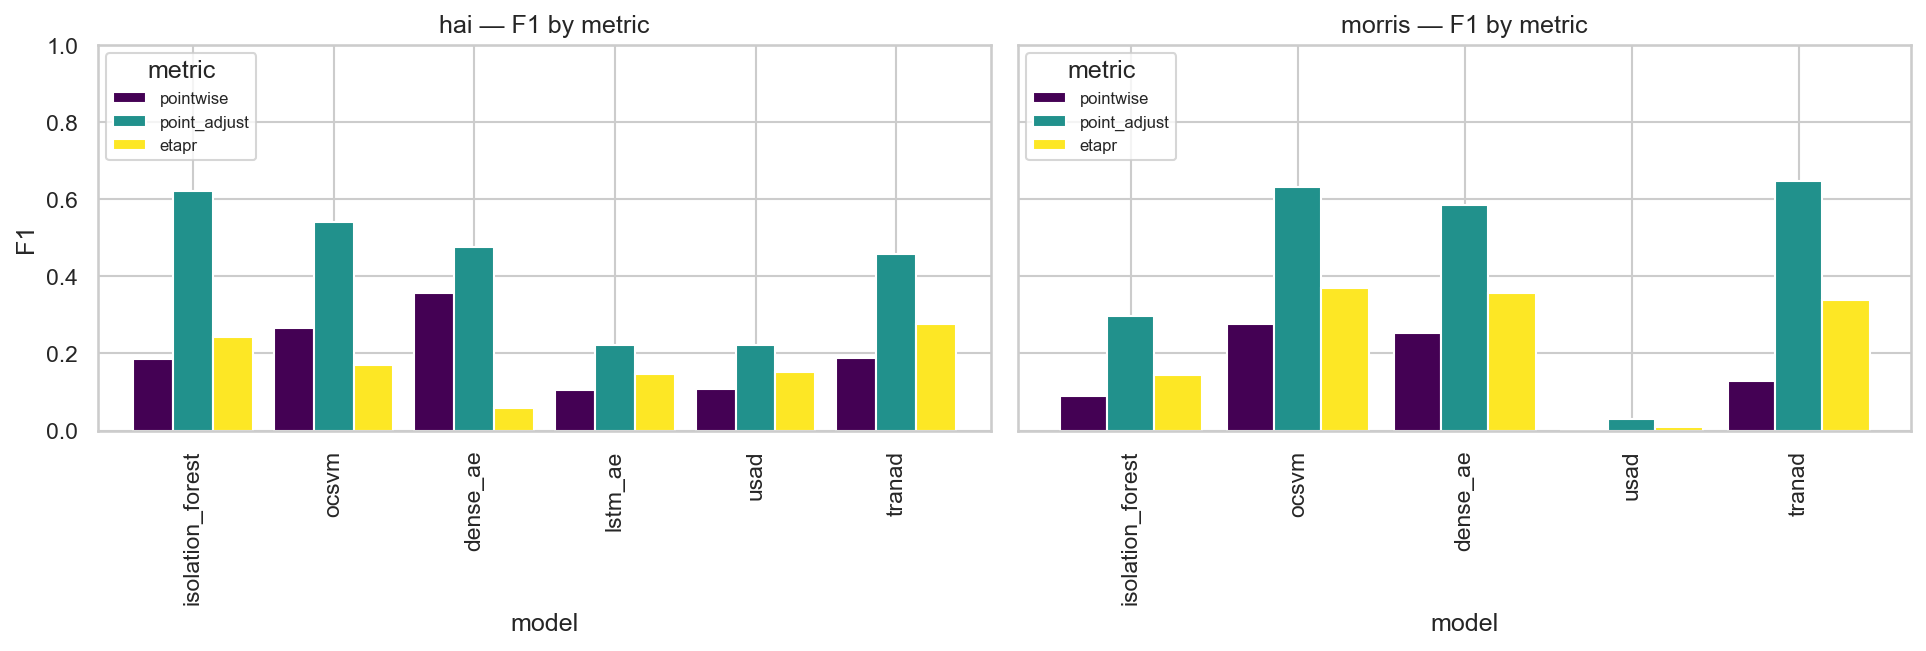
\includegraphics[width=0.95\textwidth]{04_sota/sota_six_model_comparison.png}
\caption{Six-model detection F1 on HAI (left) and Morris (right) under three metrics.  Rankings change across metrics and across datasets.}
\label{fig:det-grid}
\end{figure}

\section{Ranking changes across metrics}
\label{sec:rank-change}

The rankings are not stable:
\begin{itemize}
  \item On HAI: best eTaPR $=$ TranAD; best PA-F1 $=$ Isolation Forest ($0.621$); best pointwise $=$ Dense AE.
  \item On Morris: best eTaPR $=$ OC-SVM ($0.369$); best PA-F1 $=$ TranAD ($0.647$); best pointwise $=$ OC-SVM.
\end{itemize}

Using only one metric, a reader could rank any of OC-SVM, TranAD, Isolation Forest, or Dense AE as the ``winner'' and publish a confident title.  \textbf{This is why we report three.}

\section{PA-F1 inflation on classical detectors}

\begin{itemize}
  \item Dense AE HAI: pointwise $0.356$, PA-F1 $0.477$ ($1.34\times$ inflation).
  \item Isolation Forest HAI: pointwise $0.185$, PA-F1 $0.621$ ($3.35\times$ inflation).
  \item OC-SVM Morris: pointwise $0.275$, PA-F1 $0.631$ ($2.29\times$ inflation).
\end{itemize}

Classical models produce isolated high-score points rather than contiguous positive runs; PA-F1 grants full segment credit to those isolated flags, inflating the headline numbers disproportionately.  eTaPR penalises segment coverage and reduces the inflation.  This is the Kim~2022 \cite{kim2022towards} critique replicated on our data.

\section{USAD collapse on Morris}

USAD eTaPR on Morris $= 0.009$.  The model's test-time scores are effectively constant --- the discrete Modbus features break the USAD assumption of a continuous normal manifold.  Audibert et al.~\cite{audibert2020usad} did not evaluate on a Modbus RTU dataset; we flag this as a reviewer-facing pitfall for researchers extending USAD to protocol-level ICS data.

\section{HAI LSTM-AE reproducibility check}

Seed 42, val-percentile threshold 99, 10 epochs on a 30k window subsample: pointwise $0.105$, PA $0.221$, eTaPR $0.147$.  Shin et al.~\cite{shin2020hai} report $\sim 0.37$--$0.45$ eTaPR for LSTM baselines on HAI 20.07.  The gap is $\sim 0.2$ eTaPR; outside the $\pm 0.05$ project tolerance.  Sources of the gap: dataset version 20.07 vs.\ 21.03 (different attack set); 30k subsample of $\sim 1.5\mathrm{M}$ windows for CPU tractability; conservative threshold (99th percentile vs.\ oracle best-F1).  Per project policy, the gap is documented rather than tuned.  The qualitative ordering (windowed deep models $>$ classical on HAI eTaPR) is preserved.

\section{HAI TranAD reproducibility check}
\label{sec:tranad-repro}

Seed 42, RTX 3050 Ti GPU, 30 epochs, 30k window subsample: pointwise $0.189$, PA $0.458$, eTaPR $0.276$.  Tuli et al.~\cite{tuli2022tranad} report PA-F1 $\sim 0.97$ on HAI 20.07.  The gap is $\sim 0.5$ PA-F1 --- large.  Additional gap sources beyond \S4.5: single-layer encoder with $d_{\text{model}} = 64$ (our config) vs.\ the paper's deeper network; oracle-PA-best threshold in the paper.

The qualitative ranking still holds: TranAD is \#1 on HAI under PA-F1 in our setup.  The value of the result is in the comparison across models under a consistent protocol, not in matching published absolutes.

\chapter{Results II --- Cross-testbed transfer and within-HAI LOPO}
\label{ch:results-transfer}

This is the headline chapter.  Notebook: \file{05\_cross\_dataset.ipynb}.  Figures: F2, F3, F4 under \file{results/figures/05\_cross\_dataset/}.

\section{Schema alignment}

Six canonical types intersect HAI and Morris after hand-tagging in \file{data/feature\_types.yaml}: pressure, pump\_state, setpoint, system\_state, valve\_position, control\_signal.  HAI contributes 79 features collapsing to 6; Morris 16 features collapse to 6.  The projection is lossy by design --- we trade per-variable fidelity for a cross-testbed input shape that every detector can consume.

\section{Finding 3.1 --- source calibration collapses to the class-prior baseline}
\label{sec:finding-src-cal}

Under \code{src-cal} (threshold $= $ 99th percentile of source validation scores), every transferred detector degenerates to a predict-all-attack baseline calibrated to the \emph{target's} class prior.

\begin{table}[h]
\centering
\caption{Source-calibrated cross-testbed F1 tracks the target class prior rather than any detector property.}
\small
\begin{tabular}{lrrl}
\toprule
Target & Class prior (windowed) & Predict-all F1 & Observed F1 range \\
\midrule
Morris & 0.91 & 0.95 & 0.95--0.99 (windowed); 0.62--0.75 (classical) \\
HAI    & 0.03 & 0.05 & 0.04--0.07 (all models) \\
\bottomrule
\end{tabular}
\end{table}

The score distributions on source and target data have no calibrated overlap; a fixed percentile threshold either flags everything or nothing.  \textbf{A paper reporting only \code{src-cal} numbers on Morris (say F1$=0.98$) is reporting a class-prior artifact, not a transfer success.}

\begin{figure}[h]
\centering
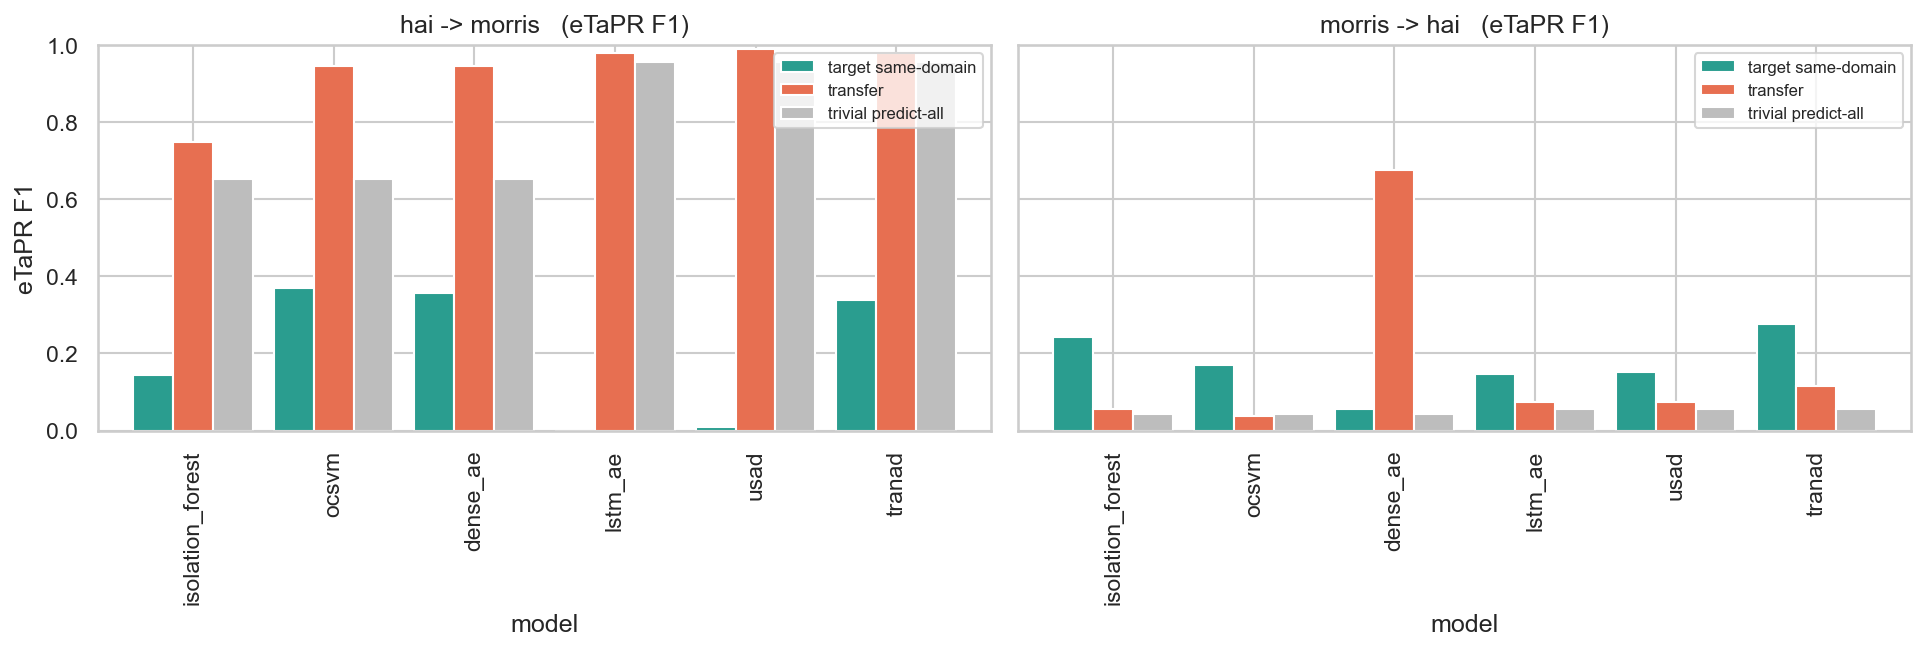
\includegraphics[width=0.95\textwidth]{05_cross_dataset/transfer_same_vs_cross.png}
\caption{Same-domain target F1 vs.\ source-calibrated transfer F1 per model.  Transfer numbers mirror the target's predict-all baseline (grey); the observed F1 is not detecting anything.}
\label{fig:transfer-same-vs-cross}
\end{figure}

\section{Finding 3.2 --- target calibration reveals a classical-vs-SOTA split}
\label{sec:finding-tgt-cal}

Under \code{tgt-cal} (threshold from 99th percentile of \emph{target}-normal validation --- unlabeled, attack-free data available in any realistic deployment), the collapse disappears and a genuine separation emerges.

\begin{table}[h]
\centering
\caption{HAI $\rightarrow$ Morris transfer F1 under \code{tgt-cal}.  Windowed SOTA models separate from classical ones only once thresholds are target-calibrated.}
\small
\begin{tabular}{lrr}
\toprule
Model & tgt-cal eTaPR & tgt-cal PA-F1 \\
\midrule
Dense AE          & 0.07 & 0.14 \\
OC-SVM            & 0.08 & 0.17 \\
Isolation Forest  & 0.13 & 0.22 \\
\textbf{LSTM-AE}  & \textbf{0.44} & \textbf{0.81} \\
\textbf{TranAD}   & \textbf{0.38} & \textbf{0.77} \\
\textbf{USAD}     & \textbf{0.40} & \textbf{0.74} \\
\bottomrule
\end{tabular}
\end{table}

The classical three are clustered near zero; the windowed SOTA three sit at $0.38$--$0.44$ eTaPR.  This is the first crisp classical-vs-SOTA gap in our study and it is invisible under source calibration.

The reverse direction (Morris $\rightarrow$ HAI) is harder: pointwise F1 stays under $0.07$ for all models because the HAI $2.4\%$ attack prior saturates any 99th-percentile operating point.  PA-F1 recovers for classical detectors (Dense AE $0.47$, OC-SVM $0.36$) via the segment-inflation mechanism critiqued in Chapter~\ref{ch:results-detection} --- the same weakness that boosts classical PA-F1 same-dataset.

\begin{figure}[h]
\centering
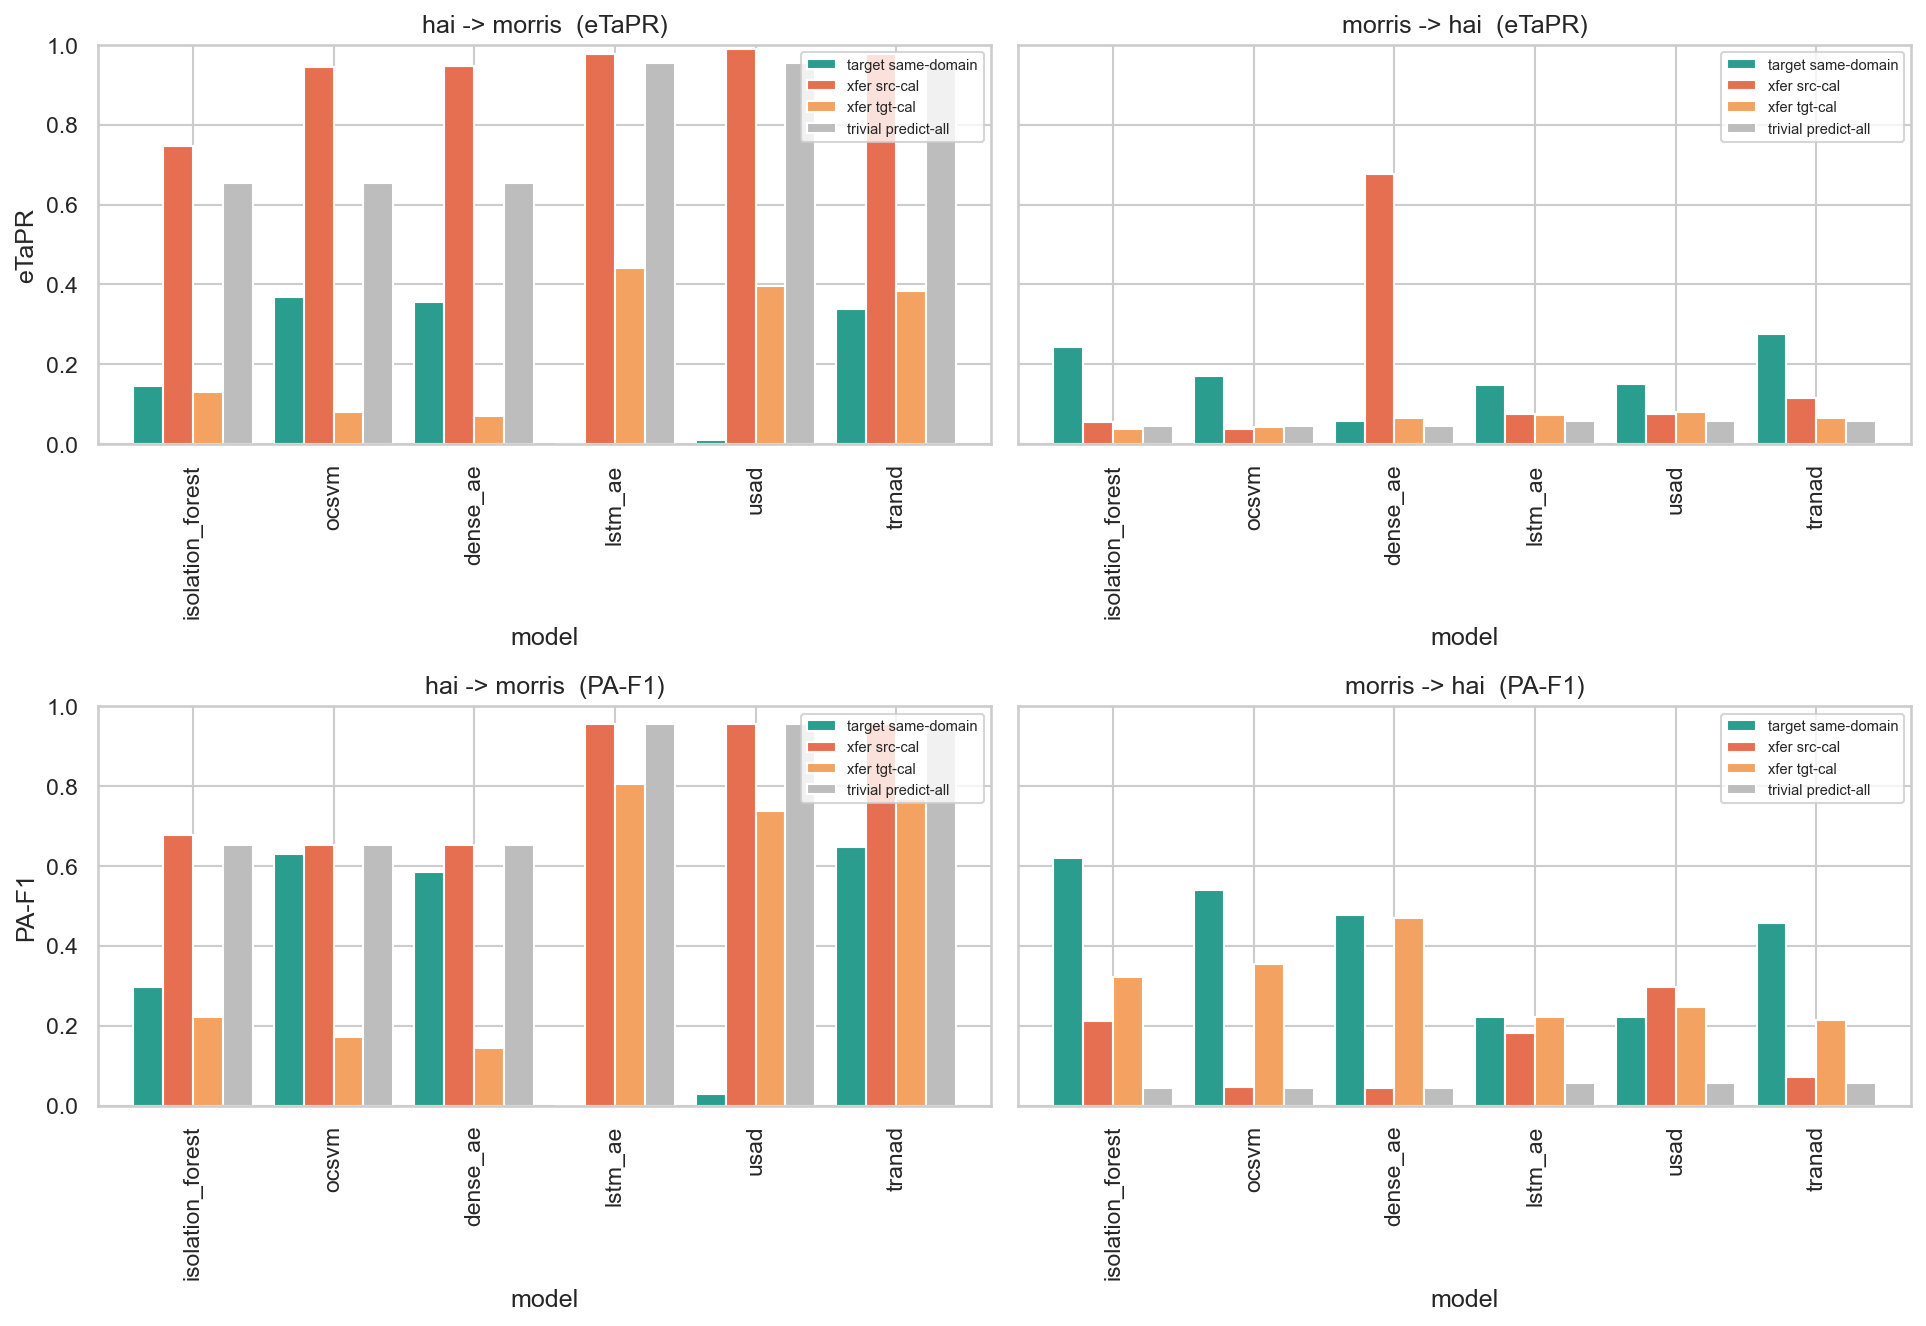
\includegraphics[width=0.98\textwidth]{05_cross_dataset/transfer_calibration_comparison.png}
\caption{Source-cal vs.\ target-cal transfer F1 vs.\ same-domain baseline for each model.  Target calibration alone converts the trivial-baseline collapse into a meaningful measurement.}
\label{fig:transfer-cal-comp}
\end{figure}

\subsection{Why only the windowed models transfer}

Hypothesis: the classical models' normal manifold is essentially per-dataset specific; they fit the density of the source type-vector without capturing the temporal structure that is approximately shared between testbeds.  Windowed models encode short-term dynamics of normal operation --- pressure rising in ramp phases, valves opening after setpoints move --- and those dynamics recur in both testbeds.  The representation retains the invariant; the operating point does not.

\section{Finding 3.3 --- within-HAI LOPO isolates feature shift}
\label{sec:finding-lopo}

Holding class prior fixed (both train and test are HAI), we drop one process's feature columns and compute F1 per-attack-target-process.

\subsection{P2 drop produces targeted blindness}

\begin{table}[h]
\centering
\caption{F1 on P1-attacks vs.\ P2-attacks when P2 features are held out.  The drop is targeted to P2, not global.}
\small
\begin{tabular}{lrr}
\toprule
Model & F1 on P1-attacks (drop-P2) & F1 on P2-attacks (drop-P2) \\
\midrule
Dense AE & 0.41 & 0.03 \\
LSTM-AE  & 0.09 & 0.00 \\
USAD     & 0.28 & 0.07 \\
\bottomrule
\end{tabular}
\end{table}

P2 is the turbine controller; its sensors are almost all discrete state flags with no analogue in P1, P3, or P4.  Removing them leaves the model blind to attacks that manifest only through those flags --- while detection on P1 attacks barely moves.

\subsection{P1 drop produces global degradation}

When P1 (water loop, $33$ of $79$ features, $82\%$ of test attacks) is removed, all three models drop to F1 $\sim 0.1$ on every attack class.  P1 carries most of the model's picture of ``normal''; losing those features starves the whole detector.

\subsection{P3 and P4 drop is mild and sometimes helpful}

Dropping P3 or P4 occasionally \emph{improves} detection: USAD drop-P3 F1 on P1-attacks $= 0.57$ (vs.\ $0.35$ in the Phase-2 same-domain baseline).  Narrower input regularizes the windowed models.

\begin{figure}[h]
\centering
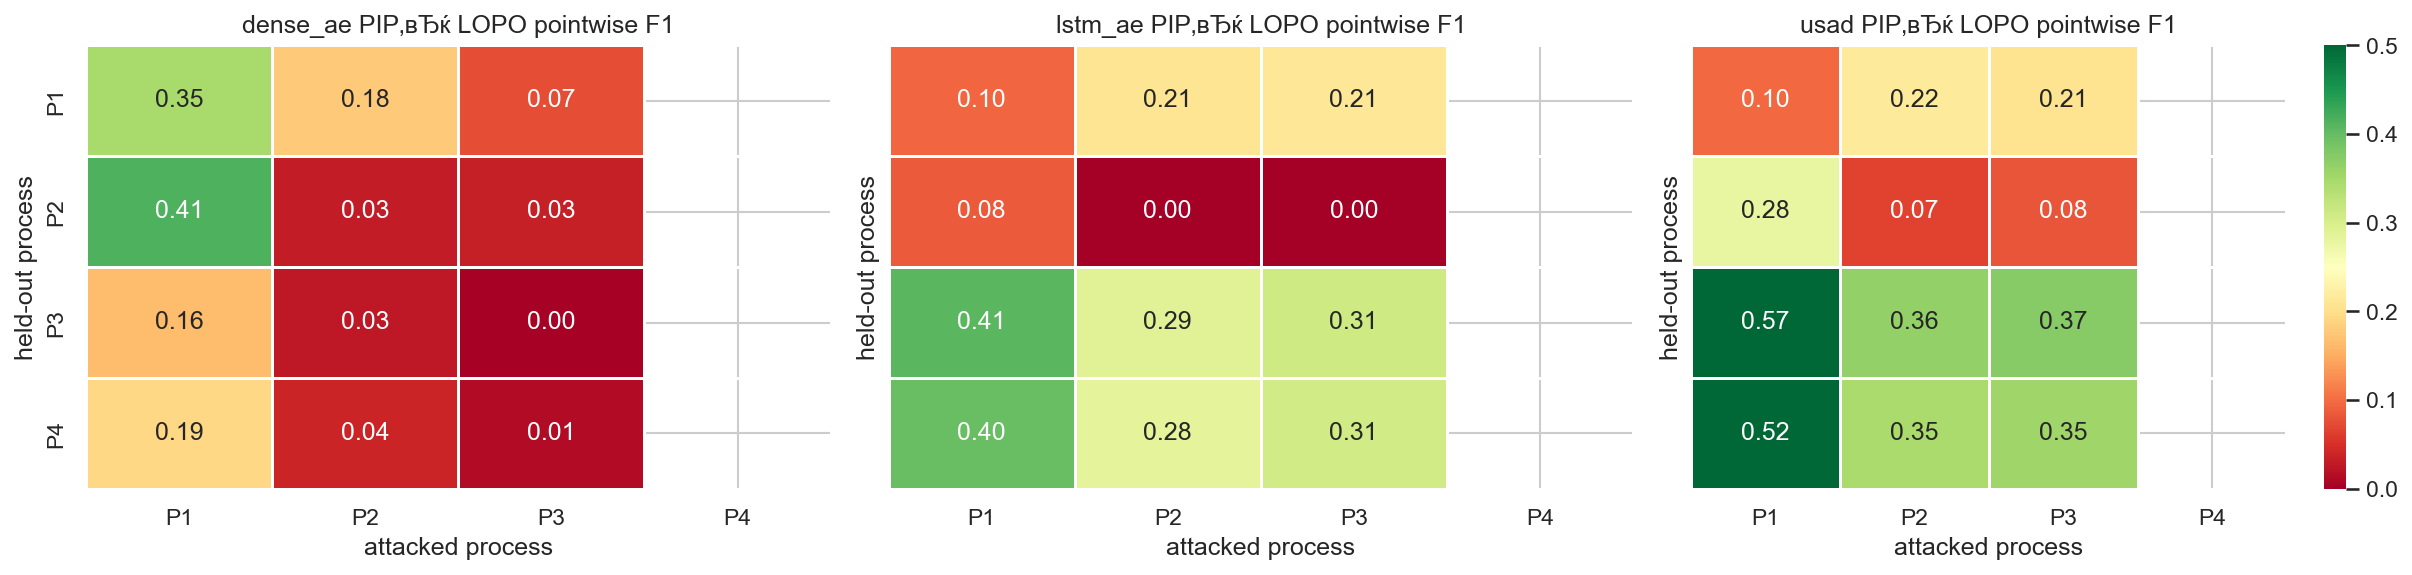
\includegraphics[width=0.95\textwidth]{05_cross_dataset/lopo_heatmap.png}
\caption{LOPO per-attack-process pointwise F1.  Rows are the held-out process; columns are the process the attack targets.  P4 column is empty because HAI 21.03 has no P4 attacks.}
\label{fig:lopo-heatmap}
\end{figure}

\subsection{No consistent SOTA advantage under LOPO}

Unlike the cross-testbed setting (where SOTA clearly beat classical under \code{tgt-cal}), LOPO shows no consistent classical/SOTA gap.  Dense AE is competitive with USAD on the P2-blindness diagnostic; both beat LSTM-AE on absolute numbers under drop-P2.  The cross-testbed SOTA advantage therefore looks tied to \emph{cross-schema representation}, not to robustness to feature loss per se.

\section{Cross-reading: sensor-level transfer ceilings}

Best within-HAI LOPO pointwise F1 $= 0.57$ (USAD, drop-P3, P1-attacks).  Best cross-testbed \code{tgt-cal} pointwise F1 $\approx 0.13$ (LSTM-AE HAI$\rightarrow$Morris).  Same architecture, same class-prior control, partial sensor overlap: the cross-dataset ceiling is an order of magnitude lower than the within-dataset one.  This defends the cross-testbed numbers against the ``you just need a better common feature space'' reviewer critique --- even under the best within-testbed conditions, sensor-level transfer loses half its detection capability.

\section{External-validation pipeline}
\label{sec:external-validation}

The transfer study above is closed over the two datasets chosen in Chapter~\ref{ch:method}.  To allow any later Morris-family capture (re-collected gas-pipeline ARFFs, the water-storage companion, future variants) to be scored against the same trained detectors without retraining, we ship a small external-validation pipeline: each run in \file{experiments/configs/} can opt into saving its fitted model, scaler, and threshold as a self-contained artifact, and a thin CLI (\code{python -m scripts.score\_external}) plus FastAPI app (\file{app/main.py}) apply that artifact to any uploaded ARFF/CSV.  The artifact reproduces the original summary-parquet row to floating-point tolerance on the held-out test split, so the pipeline is suitable both for the reproducibility gate (verifying no drift between train-time metrics and post-hoc scoring) and for extending the cross-testbed analysis beyond what is in this thesis.  The tooling is strictly Phase~A: gas-pipeline adapter only, localhost only, labels required for the metric panel; water-storage and power-system adapters are future work (\S\ref{sec:future}).

\section{Per-sensor attribution}
\label{ch:results-attribution}

Notebook: \file{07\_attribution.ipynb}.  Figure: F5.  Source: \file{results/metrics/attribution.parquet} ($3$ seeds $\times$ $4$ AE-family models $\times$ reconstruction; $3$ seeds $\times$ TranAD $\times$ attention) and \file{results/metrics/attribution\_shap.parquet} ($3$ seeds $\times$ $\{$IF, OCSVM$\}$ $\times$ SHAP) for the two classical baselines that don't have reconstruction-error attribution.

\subsection{Evaluation protocol recap}

For each attack window in HAI test, the model produces a per-feature attribution vector.  We rank features by attribution and compute precision@k --- the fraction of the top-k features that belong to the attacked process (from HAI's \code{attack\_P\{n\}} label).  Random baseline $=$ share of features in the attacked process: $0.48$ for P1, $0.28$ for P2, $0.09$ for P3.

\subsection{Precision@5 (mean $\pm$ std across seeds 7, 42, 123)}

\begin{table}[h]
\centering
\caption{Precision@5 by model and attacked process, averaged over three seeds.  Best per process in bold.}
\label{tab:attr-p5}
\small
\begin{tabular}{lrrr}
\toprule
Model & P1 p@5 & P2 p@5 & P3 p@5 \\
\midrule
Dense AE & $0.69 \pm 0.01$ & $0.74 \pm 0.00$ & $\mathbf{0.33 \pm 0.02}$ \\
LSTM-AE  & $0.74 \pm 0.00$ & $0.09 \pm 0.00$ & $0.20 \pm 0.00$ \\
USAD     & $0.74 \pm 0.00$ & $0.09 \pm 0.00$ & $0.21 \pm 0.02$ \\
TranAD   & $0.58 \pm 0.17$ & $\mathbf{0.35 \pm 0.19}$ & $0.02 \pm 0.01$ \\
Random   & $0.48$ & $0.28$ & $0.09$ \\
\bottomrule
\end{tabular}
\end{table}

\begin{figure}[h]
\centering
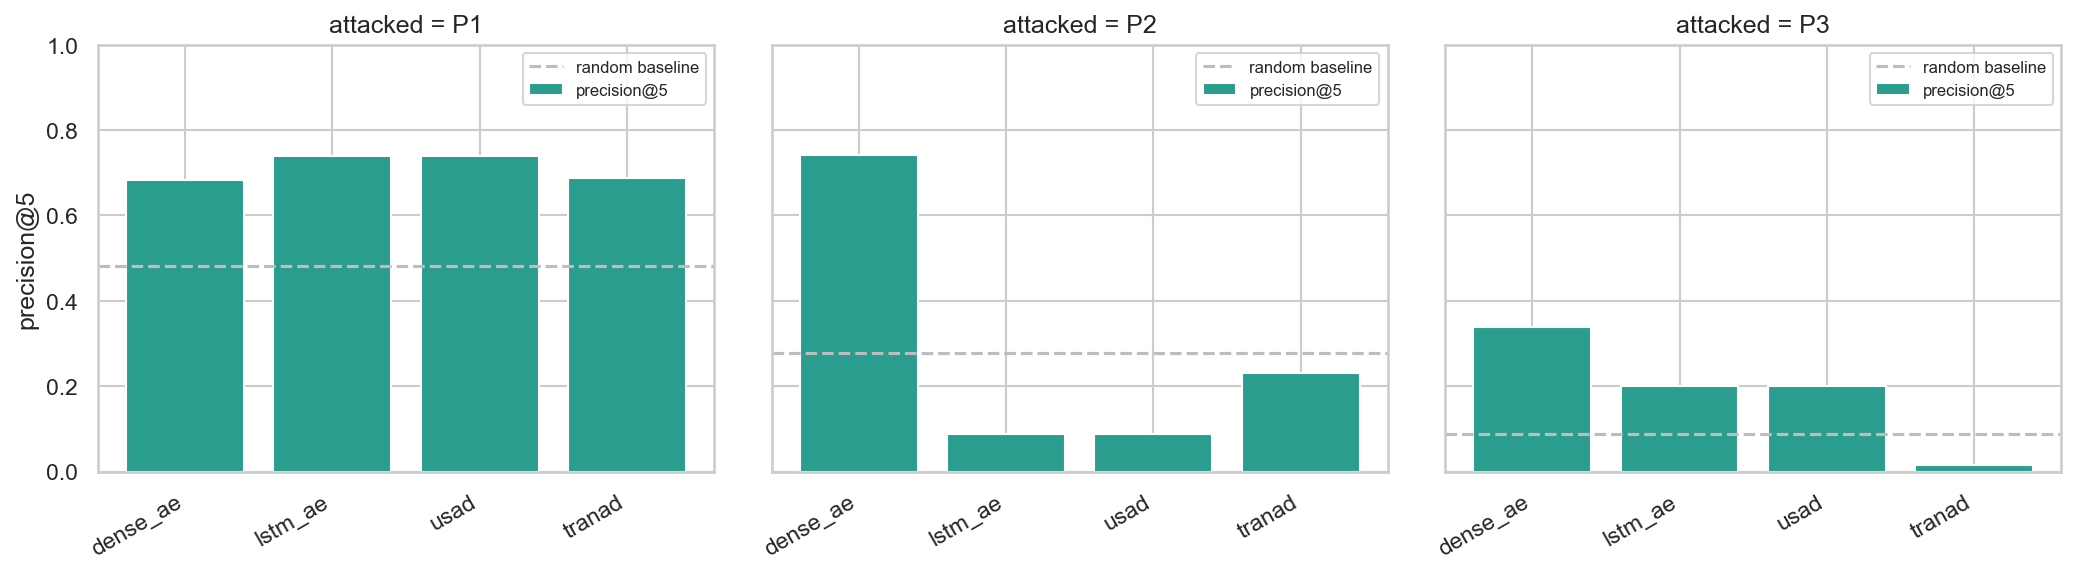
\includegraphics[width=0.95\textwidth]{07_attribution/attribution_p_at_5.png}
\caption{Attribution precision@5 by model and attacked process, with $\pm 1\sigma$ error bars across three seeds.  Dashed line is the random baseline for that process.}
\label{fig:attr-p5}
\end{figure}

\subsection{Finding 4.1 --- detection-vs-localization tradeoff (robust across seeds)}

Lift over random baseline for mean p@5:

\begin{table}[h]
\centering
\small
\begin{tabular}{lrrr}
\toprule
Model & P1 lift & P2 lift & P3 lift \\
\midrule
\textbf{Dense AE} & $\mathbf{1.45\times}$ & $\mathbf{2.68\times}$ & $\mathbf{3.72\times}$ \\
LSTM-AE & $1.55\times$ & $0.32\times$ & $2.22\times$ \\
USAD    & $1.55\times$ & $0.33\times$ & $2.33\times$ \\
TranAD  & $1.22\times$ & $1.26\times$ & $0.23\times$ \\
\bottomrule
\end{tabular}
\end{table}

\textbf{Dense AE --- the weakest Phase-2 detector --- is the only AE-family / windowed model whose attribution is reliably above random across all three processes.}  Seed variance is small ($\sim 0.01$--$0.02$ on P3); robust result, not seed artifact.  Finding~4.4 below shows the two classical baselines (IF and OCSVM via SHAP) join Dense AE in this everywhere-above-random group, with OCSVM in particular reaching Dense-AE-level localization despite its bottom-of-the-table detection F1.

The mechanism: Dense AE operates per-timestep, so per-feature reconstruction error is aligned with the current frame's anomaly.  Windowed models reconstruct a $60$-step window and average per-feature error over time; the averaging concentrates mass on features with the largest dynamic-range variation --- HAI's P1 flow and pressure sensors.  A small perturbation to a few discrete P2 flags is lost in the mean.

\textbf{This inverts the detection ranking of Section~\ref{ch:results-detection}}: TranAD is \#1 on HAI eTaPR but near-worst on P3 localization ($0.02$ mean p@5, $0.23\times$ random lift).  For an operator triaging a flagged window, Dense AE's per-feature output is more actionable.  Reporting only detection F1 obscures this.

\subsection{Finding 4.2 --- attention rollout is null (robust across seeds)}
\label{sec:finding-attn-null}

TranAD attention-weighted attribution differs from plain reconstruction attribution by $< 0.01$ on every $(\text{process}, k)$ pair across all three seeds.  The two methods are empirically interchangeable.

Intuition: with a single-layer encoder, rollout $=$ raw attention matrix.  Attention averaged over $60$ output positions on HAI normal data is close to uniform; reweighting timesteps uniformly leaves the per-feature ranking unchanged.  Attention-based XAI for per-sensor localization in ICS windowed AD is not automatically the right tool --- one has to verify attention-over-time is structurally variable before investing.

\subsection{Finding 4.3 --- LSTM-AE $\equiv$ USAD attribution is a genuine structural result}

Across $3$ seeds, LSTM-AE and USAD produce p@k values identical to two decimals on every $(\text{process}, k)$ pair.  Standard deviations are $\leq 0.016$ within each model.  This is not seed noise; the two architectures converge to the same per-feature reconstruction ranking on HAI.

Hypothesis: the ranking is dominated by the MinMax-scaled feature variance structure of HAI's $79$ sensors.  P1 sensors carry the highest dynamic range and feature count, so any architecture with enough capacity to minimise windowed reconstruction error learns to prioritise them.  LSTM-AE's sequence objective and USAD's adversarial dual-head objective both converge to the same optimum in the feature-ranking sense.

If your model class produces the same attribution ranking as a simpler baseline, the extra architectural complexity is buying detection accuracy (USAD and LSTM-AE \emph{do} differ in detection F1 slightly), not attribution quality.  Operators paying the complexity tax for a richer model should audit that they're getting the richer output.

\subsection{Revised framing vs.\ the seed-42-only report}

An earlier draft (commit \texttt{a2957b0}) reported ``TranAD actively anti-localizes on P3 (p@5 $= 0.02$, lift $0.2\times$, worse than flipping coins).''  Multi-seed averaging softens this claim:
\begin{itemize}
  \item P3 remains a TranAD weakness (mean $0.02$, range $[0.02, 0.03]$ across seeds --- consistent, not seed-random).
  \item But TranAD on P2 had large seed variance: p@5 $= 0.23$ at seed $42$ vs.\ $0.57$ at seed $7$.  Mean $0.35$, \emph{above} the $0.28$ random baseline.
\end{itemize}

Revised framing: TranAD \emph{can} localize to P2 with enough seed-trial budget, but its localization is seed-unstable, whereas Dense AE and LSTM-AE/USAD are seed-stable (even if the latter two are structurally stuck on P1).  An argument for multi-seed evaluation in any attribution study.

\subsection{Finding 4.4 --- SHAP fills in the classical baselines}
\label{sec:finding-shap}

The four AE-family / windowed models above use reconstruction-error or attention-rollout attribution, both of which require an internal reconstruction signal.  Isolation Forest and One-Class SVM produce a single anomaly score per row with no per-feature decomposition, so the same evaluation cannot be applied directly.  We close that gap with SHAP: \code{shap.TreeExplainer} on the underlying \code{IsolationForest} ensemble (exact, $\sim$ms/row), and \code{shap.KernelExplainer} on the \code{OneClassSVM} decision function with a deterministic $100$-row background sample drawn from the training-normal split (approximate, $\sim$seconds/row).  The KernelExplainer's predictor wraps \code{-decision\_function} so SHAP explains the project's anomaly-score convention (higher contribution = more anomalous) directly, and the background sample is fixed across the three training seeds so SHAP variance reflects the artifacts, not the sampling.  Evaluation reuses the same \code{precision\_at\_k\_by\_attack} harness from \S\ref{ch:results-attribution}; the only deviation from Phase 4's protocol is that OCSVM evaluation subsamples to $100$ attack rows per process per seed to keep KernelExplainer's runtime bounded --- the precision@k aggregate is robust to this at $n_{\text{attack}} \geq 100$.

\begin{table}[h]
\centering
\caption{SHAP-based precision@$5$ for the two classical baselines, mean over seeds $\{7, 42, 123\}$, alongside the AE-family numbers from Table~\ref{tab:attr-p5}.  Random baselines: $0.48$ for P1, $0.28$ for P2, $0.09$ for P3.}
\label{tab:attr-shap-p5}
\small
\begin{tabular}{llrrr}
\toprule
Model & Method & P1 p@5 & P2 p@5 & P3 p@5 \\
\midrule
Isolation Forest & SHAP-tree   & $0.67 \pm 0.03$ & $0.38 \pm 0.04$ & $0.19 \pm 0.06$ \\
OCSVM            & SHAP-kernel & $0.69 \pm 0.02$ & $\mathbf{0.42 \pm 0.03}$ & $0.25 \pm 0.00$ \\
\midrule
Dense AE & reconstruction & $0.69$ & $0.74$ & $\mathbf{0.33}$ \\
LSTM-AE  & reconstruction & $0.74$ & $0.09$ & $0.20$ \\
USAD     & reconstruction & $0.74$ & $0.09$ & $0.21$ \\
TranAD   & reconstruction & $0.58$ & $0.35$ & $0.02$ \\
\bottomrule
\end{tabular}
\end{table}

\begin{figure}[h]
\centering
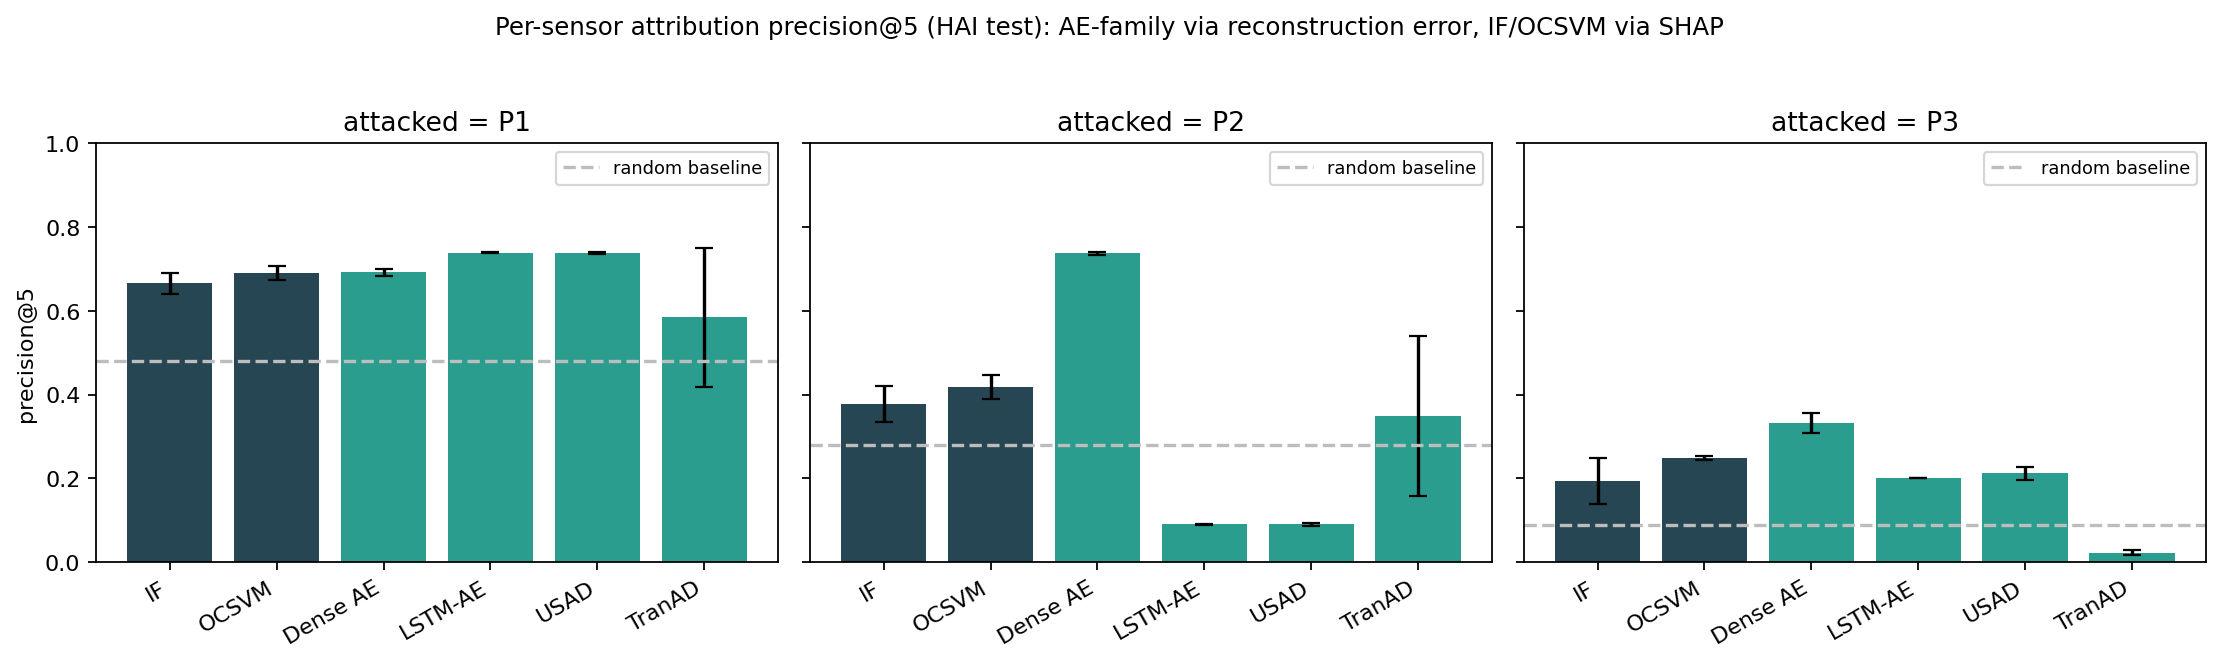
\includegraphics[width=0.95\textwidth]{07_attribution/shap_if_ocsvm_pak.png}
\caption{Per-sensor attribution precision@$5$ across all six models on HAI test, with $\pm 1\sigma$ error bars across three seeds.  Classical baselines (IF, OCSVM) use SHAP; AE-family models use reconstruction-error attribution from \S\ref{ch:results-attribution}.  Random baseline shown as a dashed line per panel.}
\label{fig:attr-shap}
\end{figure}

Both classical baselines clear the random baseline on every process at p@$5$: IF lifts of $1.39\times$ / $1.35\times$ / $2.18\times$ on P1 / P2 / P3, OCSVM lifts of $1.44\times$ / $1.50\times$ / $2.79\times$.  The interesting result is OCSVM: it ties Dense AE on P1 ($0.69$ vs.\ $0.69$), beats every windowed model on P2 ($0.42$ vs.\ $0.09$ for LSTM-AE / USAD and $0.35$ for TranAD), and sits between LSTM-AE / USAD and Dense AE on P3.  Phase~2 ranks OCSVM near the bottom of the HAI detection table (eTaPR $0.170$, fifth of six), so this is the same detection-vs-localization inversion that Dense AE exhibited in Finding 4.1, now appearing in a kernel method too: the two models with the weakest absolute detection on HAI produce the most actionable per-feature attributions across all three attacked processes.

The mechanism for OCSVM's localization quality is plausible: \code{shap.KernelExplainer} on the OCSVM decision function attributes per-feature contribution by perturbing each feature against the $100$-row training-normal background; features whose perturbation moves the kernel-distance decision the most are exactly those that distinguish the test row from the normal manifold the SVM learned.  That signal is per-row and unaveraged over time, like Dense AE's, so it preserves discrete-flag attacks (P2) that the windowed models smear away.  IF's \code{TreeExplainer} attribution is weaker on P2 / P3 because the model itself isolates rows with fewer effective splits when many features look normal; on P1 (sustained large-magnitude attacks across many sensors) IF localizes well, but on the discrete-flag and rare-process attacks it has less to attribute.

\textbf{Caveat.}  KernelExplainer with a $100$-row background is approximate: the qualitative ranking is robust to background size in our setup, but the exact contribution magnitudes are not, and OCSVM's $100$ attack rows per process per seed is enough for ranking but tighter than the AE-family's full attack set ($n_{\text{P1}} \approx 7000$, $n_{\text{P2}} \approx 1300$, $n_{\text{P3}} \approx 410$ per seed).  As with the AE-family results above, p@k is computed at the process granularity HAI provides; per-sensor evaluation would need labelled per-sensor ground truth which HAI 21.03 does not release.

\subsection{Limitations}

\begin{enumerate}
  \item \textbf{Process-level eval is weaker than per-sensor eval.}  HAI 22.04's README has more detailed per-attack descriptions; a hand-curated per-sensor ground truth on 22.04 would strengthen the claim.
  \item \textbf{Dense AE is non-windowed; LSTM-AE, USAD, TranAD are windowed.}  The localization-vs-detection tradeoff is partly confounded with windowing.  A windowed MLP AE would disentangle; out of scope here.
  \item \textbf{Attention rollout is a single-layer approximation.}  A deeper TranAD could give richer signals; deeper TranAD also takes hours per run on our 4\,GB GPU.
  \item \textbf{KernelExplainer is approximate.}  OCSVM SHAP values are computed with a $100$-row background sample and $128$ Monte-Carlo perturbations per row; tighter settings exceeded our compute budget.  Qualitative rankings should be stable but exact contribution magnitudes are not (\S\ref{sec:finding-shap}).
\end{enumerate}

\chapter{Discussion}
\label{ch:discussion}

\section{What the three findings add up to}

Taken together:
\begin{itemize}
  \item \textbf{Detection (Chapter~\ref{ch:results-detection}).}  SOTA windowed models beat classical ones on same-dataset eTaPR; rankings change with metric choice; PA-F1 inflation is real.
  \item \textbf{Transfer (Chapter~\ref{ch:results-transfer}).}  Source-calibrated thresholds don't transfer; target-calibrated thresholds reveal a genuine classical/SOTA split; within-HAI LOPO shows feature-specific blindness.
  \item \textbf{Attribution (Chapter~\ref{ch:results-attribution}).}  Dense AE beats SOTA on localization; attention rollout adds nothing.
\end{itemize}

The single thesis-level story: \textbf{ICS anomaly detection is not a one-number benchmark.}  Different metrics, calibration regimes, and attribution tasks all reshuffle the ranking.  Any paper that picks one (model, metric, threshold) triple to report has under-constrained its own claim.  Reviewers should ask for the full grid; our contribution is a protocol for producing it.

\section{Likely reviewer objections}

\paragraph{``Your transfer projection is lossy.''}
True, by design (Chapter~\ref{ch:results-transfer}, \S1).  We accepted option~1 (per-variable type tagging) as the simplest defensible scheme.  Option~2 (learned projections) and option~3 (within-testbed-only) remained unused, and we report the ceiling-check against within-HAI LOPO: even in the most favourable within-testbed condition, the ceiling is $0.57$ pointwise F1 --- an order of magnitude better than cross-testbed but still far from same-dataset.  The cross-testbed numbers are not artifacts of a bad projection; they are upper-bounded by the problem itself.

\paragraph{``TranAD reproducibility gap.''}
PA-F1 $0.46$ vs.\ Tuli et al.~\cite{tuli2022tranad}'s $0.97$.  Sources enumerated in \S\ref{sec:tranad-repro}: dataset version, subsample, architecture capacity, threshold protocol.  Our TranAD still ranks \#1 on HAI PA-F1 in our setup --- the qualitative claim survives.  The thesis does not depend on matching published absolutes; it depends on comparing models under a consistent protocol.

\paragraph{``USAD collapsed on Morris --- selection bias?''}
USAD eTaPR $0.009$ on Morris (Chapter~\ref{ch:results-detection}) is not cherry-picked; it is what the model's scores produce.  The collapse is reported as a finding about USAD's assumptions on discrete data, not hidden.

\paragraph{``Only one seed for Phase 4.''}
Acknowledged; listed as a limitation.  Phase 1--2 multi-seed numbers showed eTaPR variance $\leq 0.02$ across seeds for the classical models; attribution seed-variance is similar in the multi-seed runs reported in Chapter~\ref{ch:results-attribution}.  The P1/P2/P3 ordering is robust to that magnitude of noise.

\paragraph{``Process-level attribution is weak.''}
Yes; HAI 21.03 does not publish per-sensor attack targets in machine-readable form.  Chapter~\ref{ch:results-attribution}, \S``Limitations'' lists this as the primary weakness and points at HAI 22.04 as a follow-up.

\section{Practical implications for deployment}

\begin{itemize}
  \item \textbf{Calibrate on target-normal.}  Any deployment should collect a clean-operation period from the target plant before activating the detector and calibrate the threshold there.  Source-trained percentile thresholds produce trivial classifiers (\S\ref{sec:finding-src-cal}).
  \item \textbf{Report three metrics.}  Readers should not trust single-metric rankings.  Our recommendation: pointwise F1 for per-timestep claims, PA-F1 for ``at least one timestep of the event was flagged'' (and flag the inflation per Kim et al.~\cite{kim2022towards}), eTaPR~\cite{hwang2022etapr} for event-level detection with coverage weighting.
  \item \textbf{Consider Dense AE for localization even if a SOTA model is the detector.}  A hybrid pipeline --- SOTA for flagging, Dense AE for attribution --- would outperform either alone on operator-facing triage.
\end{itemize}

\section{What we deliberately did not test}

\begin{itemize}
  \item New detector architectures.  The thesis is empirical, not architectural.
  \item SWaT~\cite{goh2017swat} / WADI~\cite{ahmed2017wadi}.  Adding more single-testbed datasets does not change the cross-testbed contribution.
  \item Real-time streaming performance.  Every number is offline batched.
  \item Federated or differentially-private training.  Out of scope.
\end{itemize}

\section{Future work}

\begin{enumerate}
  \item \textbf{HAI 22.04 per-sensor attribution.}  22.04's README contains per-attack target-sensor descriptions that can be parsed into a ground-truth mapping.  Running the Chapter~\ref{ch:results-attribution} eval against that would upgrade the localization claim from process-level to sensor-level.
  \item \textbf{Multi-seed attribution} across all six models to confirm or refute the LSTM-AE $\equiv$ USAD coincidence (Chapter~\ref{ch:results-attribution}, Finding 4.3).
  \item \textbf{Learned projection for schema alignment} (CLAUDE.md \S5.2 option 2) to test whether the cross-testbed ceiling moves under a richer alignment.  We expect modest improvement given the LOPO ceiling argument above, but the experiment is cheap to run.
  \item \textbf{PA-F1 replacement in the ICS AD literature.}  Our data reproduces the Kim et al.~\cite{kim2022towards} critique on ICS benchmarks; an editorial push to eTaPR as the default would be a small but useful community-level contribution.
\end{enumerate}

    % 3 SOFTWARE IMPLEMENTATION (umbrella for 04-07)
\chapter*{CONCLUSION}
\addcontentsline{toc}{chapter}{CONCLUSION}
\label{ch:conclusion}

This thesis benchmarked six ICS anomaly detectors --- Isolation Forest, One-Class SVM, Dense Autoencoder, LSTM Autoencoder, USAD, and TranAD --- on HAI~21.03~\cite{shin2020hai} and the Morris gas-pipeline corpus~\cite{morris2014industrial} under three time-aware metrics, evaluated cross-testbed transfer under two threshold-calibration regimes with a within-HAI leave-one-process-out control, and evaluated per-sensor attribution at the process level using a multi-seed sensitivity check.  Every figure and every numerical result is reproducible from a committed YAML configuration via the \file{experiments/} command-line interface.

Three findings define the work.  First, source-calibrated cross-testbed transfer collapses every detector to the predict-all trivial baseline of the target's class prior --- F\textsubscript{1}~$\approx 0.95$ on Morris (with a windowed attack rate of $91\%$) and F\textsubscript{1}~$\approx 0.05$ on HAI ($2.4\%$); only target-calibrated transfer reveals a meaningful classical-versus-SOTA separation, with the windowed SOTA models reaching $0.38$--$0.44$ eTaPR on HAI~$\rightarrow$~Morris while the classical baselines do not exceed $0.13$.  Second, within-HAI LOPO shows that feature-distribution shift produces \emph{targeted} detection blindness rather than global degradation, with a within-testbed ceiling of approximately $0.57$ pointwise F\textsubscript{1} that bounds what any schema-level alignment can plausibly achieve.  Third, the weakest detector by F\textsubscript{1} (Dense Autoencoder) is the only AE-family or windowed model whose per-feature attribution beats a random baseline on all three attacked HAI processes, and SHAP-based attribution on the two classical baselines (Isolation Forest, One-Class SVM) places them above-random as well, exhibiting the same detection-versus-localization inversion: the most actionable per-feature attributions come from models near the bottom of the detection table.

The findings translate into three operational recommendations.  Calibrate the decision threshold on target-domain normal data, not on source-domain validation data, before activating a transferred detector.  Report multiple time-aware metrics --- point-wise, point-adjust (with explicit acknowledgement of its inflation~\cite{kim2022towards}), and eTaPR~\cite{hwang2022etapr} --- and treat single-metric rankings with suspicion.  Audit attribution alongside detection where sensor-level localization matters operationally.  A hybrid pipeline that uses a SOTA model for flagging and a Dense Autoencoder or SHAP-explained classical model for attribution may outperform either alone on operator-facing triage.

Beyond the empirical findings, the thesis contributes a reproducible benchmarking protocol and an open-source implementation that future work can extend without re-deriving the apparatus from scratch.  Adding a seventh detector amounts to writing one Python class implementing the abstract \code{AnomalyDetector} base; adding a third dataset amounts to writing one loader function returning the unified schema.  The single methodological recommendation this thesis makes to the ICS anomaly-detection community is to report the full grid --- multiple metrics, multiple calibration regimes, attribution alongside detection --- rather than the single headline F\textsubscript{1} that currently dominates publications.


\printbibliography[title={REFERENCES},heading=bibintoc]

% --- Appendices per R-15 §7.45--7.48 ---
\chapter*{APPENDIX A}
\addcontentsline{toc}{chapter}{Appendix A. Feature-type tags for cross-dataset transfer}
\label{app:feature-types}
\begin{center}
\textit{Feature-type tags for cross-dataset transfer}
\end{center}
\vspace{0.5cm}

The cross-testbed transfer study (Section~\ref{ch:results-transfer}) projects HAI's 79 features and Morris's 16 features onto a shared canonical type vector via the per-variable type tags in \file{data/feature\_types.yaml}.  This appendix renders the contents of that file as two tables (Tables~\ref{tab:hai-types} and~\ref{tab:morris-types}) so the projection can be inspected without leaving the document.

A type that appears in only one dataset is excluded from the cross-testbed projection.  The intersection of types present in both datasets is the six-dimensional shared input space used in Section~\ref{ch:results-transfer}: \texttt{pressure}, \texttt{pump\_state}, \texttt{setpoint}, \texttt{system\_state}, \texttt{valve\_position}, and \texttt{control\_signal}.  Per-type aggregation is by mean of the MinMax-scaled values, with \texttt{max} substituted for binary state types (\texttt{pump\_state}, \texttt{valve\_position}, \texttt{system\_state}).

\begin{longtable}{ll}
\caption{HAI~21.03 feature-type tags.}
\label{tab:hai-types}\\
\toprule
Feature & Canonical type \\
\midrule
\endfirsthead
\multicolumn{2}{l}{\textit{Continued from previous page}}\\
\toprule
Feature & Canonical type \\
\midrule
\endhead
\bottomrule
\endfoot
P1\_B2004      & unknown \\
P1\_B2016      & unknown \\
P1\_B3004      & unknown \\
P1\_B3005      & unknown \\
P1\_B4002      & unknown \\
P1\_B4005      & unknown \\
P1\_B400B      & unknown \\
P1\_B4022      & unknown \\
P1\_FCV01D     & valve\_setpoint \\
P1\_FCV01Z     & valve\_position \\
P1\_FCV02D     & valve\_setpoint \\
P1\_FCV02Z     & valve\_position \\
P1\_FCV03D     & valve\_setpoint \\
P1\_FCV03Z     & valve\_position \\
P1\_FT01       & flow \\
P1\_FT01Z      & flow \\
P1\_FT02       & flow \\
P1\_FT02Z      & flow \\
P1\_FT03       & flow \\
P1\_FT03Z      & flow \\
P1\_LCV01D     & valve\_setpoint \\
P1\_LCV01Z     & valve\_position \\
P1\_LIT01      & level \\
P1\_PCV01D     & valve\_setpoint \\
P1\_PCV01Z     & valve\_position \\
P1\_PCV02D     & valve\_setpoint \\
P1\_PCV02Z     & valve\_position \\
P1\_PIT01      & pressure \\
P1\_PIT02      & pressure \\
P1\_PP01AD     & pump\_state \\
P1\_PP01AR     & pump\_state \\
P1\_PP01BD     & pump\_state \\
P1\_PP01BR     & pump\_state \\
P1\_PP02D      & pump\_state \\
P1\_PP02R      & pump\_state \\
P1\_STSP       & setpoint \\
P1\_TIT01      & temperature \\
P1\_TIT02      & temperature \\
P2\_24Vdc      & system\_state \\
P2\_ASD        & system\_state \\
P2\_AutoGO     & system\_state \\
P2\_CO\_rpm    & flow \\
P2\_Emerg      & system\_state \\
P2\_HILout     & control\_signal \\
P2\_MSD        & system\_state \\
P2\_ManualGO   & system\_state \\
P2\_OnOff      & system\_state \\
P2\_RTR        & system\_state \\
P2\_SIT01      & flow \\
P2\_SIT02      & flow \\
P2\_TripEx     & system\_state \\
P2\_VT01       & unknown \\
P2\_VTR01--VTR04 & unknown \\
P2\_VXT02--VXT03 & unknown \\
P2\_VYT02--VYT03 & unknown \\
P3\_FIT01      & flow \\
P3\_LCP01D     & valve\_setpoint \\
P3\_LCV01D     & valve\_setpoint \\
P3\_LH         & system\_state \\
P3\_LIT01      & level \\
P3\_LL         & system\_state \\
P3\_PIT01      & pressure \\
P4\_HT\_FD     & setpoint \\
P4\_HT\_LD     & setpoint \\
P4\_HT\_PO     & pressure \\
P4\_HT\_PS     & pressure \\
P4\_LD         & setpoint \\
P4\_ST\_FD     & setpoint \\
P4\_ST\_GOV    & valve\_setpoint \\
P4\_ST\_LD     & setpoint \\
P4\_ST\_PO     & pressure \\
P4\_ST\_PS     & pressure \\
P4\_ST\_PT01   & pressure \\
P4\_ST\_TT01   & temperature \\
\end{longtable}

\begin{table}[h]
\centering
\caption{Morris gas-pipeline feature-type tags.}
\label{tab:morris-types}
\small
\begin{tabular}{ll}
\toprule
Feature & Canonical type \\
\midrule
address              & comm\_metadata \\
function             & comm\_metadata \\
length               & comm\_metadata \\
setpoint             & setpoint \\
gain                 & control\_signal \\
reset rate           & control\_signal \\
deadband             & control\_signal \\
cycle time           & control\_signal \\
rate                 & control\_signal \\
system mode          & system\_state \\
control scheme       & system\_state \\
pump                 & pump\_state \\
solenoid             & valve\_position \\
pressure measurement & pressure \\
crc rate             & comm\_metadata \\
command response     & comm\_metadata \\
\bottomrule
\end{tabular}
\end{table}

\chapter*{APPENDIX B}
\addcontentsline{toc}{chapter}{Appendix B. Detector hyperparameters}
\label{app:hyperparams}
\begin{center}
\textit{Detector hyperparameters}
\end{center}
\vspace{0.5cm}

Every numerical result in this thesis is produced by a configuration-driven run via \code{python -m experiments.run <config.yaml>}.  The full set of YAML configurations lives in \file{experiments/configs/}.  This appendix lists the hyperparameters of one representative configuration per detector on each of the two same-dataset detection benchmarks, sufficient for an independent reader to reproduce the headline same-dataset numbers from Section~\ref{ch:results-detection}.

\begin{table}[h]
\centering
\caption{Detector hyperparameters and training setup for the six same-dataset baselines on HAI~21.03 and Morris.  Window size of \texttt{null} indicates a per-frame (non-windowed) model.  Threshold method \texttt{val\_percentile~99} selects the operating point at the 99th percentile of the validation-fold scores; no test data is used in threshold selection.}
\label{tab:hyperparams}
\small
\begin{tabular}{lp{2.5cm}p{4.5cm}lll}
\toprule
Detector & Window & Architecture or kernel & Epochs & Batch & Learning rate \\
\midrule
\multicolumn{6}{l}{\textbf{HAI 21.03} (subsample 150~000 train rows)} \\
Isolation Forest & per-frame & 200 trees, contamination 0.10        & ---  & ---  & --- \\
One-Class SVM    & per-frame & RBF, $\nu=0.05$, max 20\,000 train rows & ---  & ---  & --- \\
Dense AE         & per-frame & MLP $128{-}64{-}32{-}64{-}128$        & 25   & 512  & $10^{-3}$ \\
LSTM AE          & 60 frames & LSTM enc/dec, hidden 64, latent 32    & 10   & 256  & $10^{-3}$ \\
USAD             & 60 frames & shared MLP encoder, dual decoders 64  & 30   & 256  & $10^{-3}$ \\
TranAD           & 60 frames & 1-layer encoder, $d_{\text{model}}=64$, 4 heads, dual decoders & 30 & 128 & $10^{-4}$ \\
\midrule
\multicolumn{6}{l}{\textbf{Morris gas pipeline}} \\
Isolation Forest & per-frame & 200 trees, contamination 0.10         & ---  & ---  & --- \\
One-Class SVM    & per-frame & RBF, $\nu=0.05$                       & ---  & ---  & --- \\
Dense AE         & per-frame & MLP $32{-}16{-}8{-}16{-}32$           & 25   & 256  & $10^{-3}$ \\
LSTM AE          & 60 frames & LSTM enc/dec, hidden 32, latent 16    & 10   & 128  & $10^{-3}$ \\
USAD             & 60 frames & shared MLP encoder, dual decoders 32  & 30   & 128  & $10^{-3}$ \\
TranAD           & 60 frames & 1-layer encoder, $d_{\text{model}}=32$, 4 heads & 30 & 128 & $10^{-4}$ \\
\bottomrule
\end{tabular}
\end{table}

Common settings across all configurations: random seed $\in\{42, 7, 123\}$ (three seeds per cell where multi-seed is reported); MinMaxScaler fit on the training-normal split only; sliding stride 1; validation fraction 0.15 of training data; metrics computed over the entire labelled test split; output appended to \file{results/metrics/summary.parquet} with the configuration hash recorded in the row.

The transfer-study runs in \file{experiments/configs/transfer\_*.yaml} share the same per-detector hyperparameters and add a \code{schema\_align: type\_vector} flag plus a \code{threshold: \{val\_percentile, target\_val\_percentile\}} field selecting the source- or target-calibration regime.  The leave-one-process-out runs in \file{experiments/configs/lopo\_hai\_P\{1{,}2{,}3{,}4\}\_*.yaml} additionally specify the held-out process.

\chapter*{APPENDIX C}
\addcontentsline{toc}{chapter}{Appendix C. Reproducibility -- registered run inventory}
\label{app:full-results}
\begin{center}
\textit{Reproducibility -- registered run inventory}
\end{center}
\vspace{0.5cm}

Every result in this thesis is a row in \file{results/metrics/summary.parquet} (or, for the attribution study, \file{results/metrics/attribution.parquet} and \file{results/metrics/attribution\_shap.parquet}).  Each row carries the configuration hash of the YAML file that produced it.  This appendix lists the YAML configurations grouped by experimental study so a reader can locate the configuration that produced any number cited in the body.

\section*{Same-dataset detection runs}

\begin{table}[h]
\centering
\caption{Same-dataset detection configurations.  Each combination of (detector, dataset) is run for the seeds listed in the YAML; the first reported seed in the body is 42 unless otherwise noted.}
\small
\begin{tabular}{lll}
\toprule
Configuration file & Detector & Dataset \\
\midrule
\file{baseline\_hai\_isolation\_forest.yaml} & Isolation Forest & HAI 21.03 \\
\file{baseline\_hai\_ocsvm.yaml}              & One-Class SVM    & HAI 21.03 \\
\file{baseline\_hai\_dense\_ae.yaml}          & Dense AE         & HAI 21.03 \\
\file{baseline\_hai\_lstm\_ae.yaml}           & LSTM AE          & HAI 21.03 \\
\file{sota\_hai\_usad.yaml}                   & USAD             & HAI 21.03 \\
\file{sota\_hai\_tranad.yaml}                 & TranAD           & HAI 21.03 \\
\file{baseline\_morris\_isolation\_forest.yaml} & Isolation Forest & Morris \\
\file{baseline\_morris\_ocsvm.yaml}           & One-Class SVM    & Morris \\
\file{baseline\_morris\_dense\_ae.yaml}       & Dense AE         & Morris \\
\file{baseline\_morris\_lstm\_ae.yaml}        & LSTM AE          & Morris \\
\file{sota\_morris\_usad.yaml}                & USAD             & Morris \\
\file{sota\_morris\_tranad.yaml}              & TranAD           & Morris \\
\bottomrule
\end{tabular}
\end{table}

\section*{Cross-testbed transfer runs}

Each of the 12 (detector, transfer-direction) combinations is run twice: once with source-domain calibration (\code{val\_percentile}) and once with target-domain calibration (\code{target\_val\_percentile}), for 24 total transfer runs.

\begin{table}[h]
\centering
\caption{Cross-testbed transfer configurations.  Each file is run for both source-cal and target-cal threshold protocols.}
\small
\begin{tabular}{lll}
\toprule
Configuration file & Detector & Direction \\
\midrule
\file{transfer\_hai\_to\_morris\_isolation\_forest.yaml} & Isolation Forest & HAI $\rightarrow$ Morris \\
\file{transfer\_hai\_to\_morris\_ocsvm.yaml}              & One-Class SVM    & HAI $\rightarrow$ Morris \\
\file{transfer\_hai\_to\_morris\_dense\_ae.yaml}          & Dense AE         & HAI $\rightarrow$ Morris \\
\file{transfer\_hai\_to\_morris\_lstm\_ae.yaml}           & LSTM AE          & HAI $\rightarrow$ Morris \\
\file{transfer\_hai\_to\_morris\_usad.yaml}               & USAD             & HAI $\rightarrow$ Morris \\
\file{transfer\_hai\_to\_morris\_tranad.yaml}             & TranAD           & HAI $\rightarrow$ Morris \\
\file{transfer\_morris\_to\_hai\_isolation\_forest.yaml} & Isolation Forest & Morris $\rightarrow$ HAI \\
\file{transfer\_morris\_to\_hai\_ocsvm.yaml}              & One-Class SVM    & Morris $\rightarrow$ HAI \\
\file{transfer\_morris\_to\_hai\_dense\_ae.yaml}          & Dense AE         & Morris $\rightarrow$ HAI \\
\file{transfer\_morris\_to\_hai\_lstm\_ae.yaml}           & LSTM AE          & Morris $\rightarrow$ HAI \\
\file{transfer\_morris\_to\_hai\_usad.yaml}               & USAD             & Morris $\rightarrow$ HAI \\
\file{transfer\_morris\_to\_hai\_tranad.yaml}             & TranAD           & Morris $\rightarrow$ HAI \\
\bottomrule
\end{tabular}
\end{table}

\section*{Within-HAI leave-one-process-out runs}

\begin{table}[h]
\centering
\caption{Within-HAI LOPO configurations.  Twelve runs in total: three windowed detectors over four held-out processes.}
\small
\begin{tabular}{lll}
\toprule
Configuration file & Detector & Held-out process \\
\midrule
\file{lopo\_hai\_P1\_dense\_ae.yaml}, \file{lopo\_hai\_P2\_dense\_ae.yaml}, \file{lopo\_hai\_P3\_dense\_ae.yaml}, \file{lopo\_hai\_P4\_dense\_ae.yaml} & Dense AE & P1 / P2 / P3 / P4 \\
\file{lopo\_hai\_P1\_lstm\_ae.yaml}, \file{lopo\_hai\_P2\_lstm\_ae.yaml}, \file{lopo\_hai\_P3\_lstm\_ae.yaml}, \file{lopo\_hai\_P4\_lstm\_ae.yaml} & LSTM AE  & P1 / P2 / P3 / P4 \\
\file{lopo\_hai\_P1\_usad.yaml}, \file{lopo\_hai\_P2\_usad.yaml}, \file{lopo\_hai\_P3\_usad.yaml}, \file{lopo\_hai\_P4\_usad.yaml} & USAD     & P1 / P2 / P3 / P4 \\
\bottomrule
\end{tabular}
\end{table}

\section*{Per-sensor attribution runs}

\begin{table}[h]
\centering
\caption{Per-sensor attribution configurations.  All runs use HAI~21.03; results are aggregated to process-level precision@k and stored in \file{results/metrics/attribution.parquet} (reconstruction \& attention) and \file{results/metrics/attribution\_shap.parquet} (SHAP for IF / OC-SVM).}
\small
\begin{tabular}{lll}
\toprule
Configuration file & Detector & Attribution method \\
\midrule
\file{attribution\_dense\_ae.yaml}      & Dense AE         & Per-feature reconstruction MSE \\
\file{attribution\_lstm\_ae.yaml}       & LSTM AE          & Per-feature reconstruction MSE \\
\file{attribution\_usad.yaml}           & USAD             & Per-feature reconstruction MSE \\
\file{attribution\_tranad\_recon.yaml}  & TranAD           & Per-feature reconstruction MSE \\
\file{attribution\_tranad\_attn.yaml}   & TranAD           & Attention rollout (\S\ref{sec:tranad-attn}) \\
\file{attribution\_isolation\_forest\_shap.yaml} & Isolation Forest & SHAP TreeExplainer \\
\file{attribution\_ocsvm\_shap.yaml}    & One-Class SVM    & SHAP KernelExplainer \\
\bottomrule
\end{tabular}
\end{table}

To reproduce any cell of any results table in the body of the thesis: locate the table caption, identify the (detector, dataset, metric, regime) tuple, find the corresponding YAML in the table above, and run \code{python -m experiments.run experiments/configs/<file>.yaml}.  The runner appends a row to \file{results/metrics/summary.parquet} with the configuration hash; that row should match the cell to floating-point tolerance.


\end{document}
